% B.Tech final-year project report (black book)
% CompressKit: a latency-verified compression toolkit for convolutional neural networks
% Build:  tectonic main.tex   (run twice so the contents and figure lists settle)

\documentclass[oneside,a4paper,12pt]{report}

\usepackage[a4paper,left=1.15in,right=0.95in,top=0.95in,bottom=0.95in]{geometry}
\usepackage{amsmath}
\usepackage{etoolbox}
\usepackage{needspace}
\usepackage{tocloft}
\usepackage{titlesec}
\usepackage{graphicx}
\usepackage{fancyhdr}
\usepackage{float}
\usepackage{booktabs}
\usepackage{tabularx}
\usepackage{array}
\usepackage{multirow}
\usepackage{xcolor}
\usepackage{listings}
\usepackage{caption}
\usepackage{setspace}
\usepackage[ruled,vlined,linesnumbered]{algorithm2e}
\usepackage[nottoc,notlot,notlof]{tocbibind}
\usepackage[hidelinks]{hyperref}

\graphicspath{{figures/}}
\setcounter{secnumdepth}{3}
\setcounter{tocdepth}{1}
\setstretch{1.0}
\emergencystretch=2em
\captionsetup{font=small,labelfont=bf,skip=4pt}
\setlength{\parindent}{0mm}
\setlength{\parskip}{5pt}
\raggedbottom
\renewcommand{\arraystretch}{1.2}

\definecolor{codebg}{RGB}{246,248,247}
\definecolor{codeink}{RGB}{27,31,29}
\definecolor{codecom}{RGB}{31,122,90}
\lstset{
  basicstyle=\ttfamily\footnotesize\color{codeink},
  backgroundcolor=\color{codebg},
  commentstyle=\color{codecom},
  frame=single, rulecolor=\color{black!20},
  breaklines=true, columns=fullflexible, keepspaces=true,
  xleftmargin=2pt, xrightmargin=2pt, aboveskip=6pt, belowskip=6pt
}

\pagestyle{fancy}
\fancyhf{}
\renewcommand{\headrulewidth}{0pt}
\cfoot{\thepage}
\fancypagestyle{plain}{\fancyhf{}\renewcommand{\headrulewidth}{0pt}\cfoot{\thepage}}

% =====================================================================
%  EDIT THIS BLOCK ONLY. Every name on the cover, certificate, approval
%  sheet and acknowledgement comes from here. Items in [brackets] are
%  placeholders that must be replaced before submission.
% =====================================================================
\newcommand{\ProjectTitle}{Model Compression Toolkit}
\newcommand{\StudentA}{Relan Pratiksha Virendra}
\newcommand{\ExamA}{23054491246054}
\newcommand{\StudentB}{Joshi Bhagyesh Pradeep}
\newcommand{\ExamB}{23054491245053}
\newcommand{\StudentC}{Vora Avinash Ritesh}
\newcommand{\ExamC}{24054491245504}
\newcommand{\StudentD}{Joshi Yesha Pratik}
\newcommand{\ExamD}{24054491245512}
\newcommand{\Guide}{Dr. Kavita Patil}
\newcommand{\Hod}{Dr. Makrand Shahade}
\newcommand{\Principal}{Dr. Nilesh Salunke}
\newcommand{\Coordinator}{Dr. Kavita Patil}
\newcommand{\AcademicYear}{2026--2027}
\newcommand{\Semester}{VIII}
% =====================================================================

\makeatletter
\makeatother
\setlength{\cftbeforechapskip}{3pt}
\setlength{\cftbeforesecskip}{0pt}
\setlength{\cftbeforefigskip}{0pt}
\setlength{\cftbeforetabskip}{0pt}
\renewcommand{\cftchapfont}{\bfseries\small}
\renewcommand{\cftsecfont}{\small}
\renewcommand{\cftfigfont}{\small}
\renewcommand{\cfttabfont}{\small}
\titleformat{\chapter}[hang]{\bfseries\Large}{\thechapter.}{0.6em}{}
\titlespacing*{\chapter}{0pt}{-10pt}{14pt}
\titleformat{\section}{\bfseries\large}{\thesection}{0.6em}{}
\titlespacing*{\section}{0pt}{12pt}{4pt}
\titleformat{\subsection}{\bfseries\normalsize}{\thesubsection}{0.6em}{}
\titlespacing*{\subsection}{0pt}{9pt}{3pt}
\newcommand{\code}[1]{\texttt{\small #1}}

\begin{document}
\pagenumbering{gobble}

% ------------------------------------------------------------ cover, certificate, approval sheet
% These three pages use symmetric margins so that everything is centred on the page.
\newgeometry{left=1in,right=1in,top=0.8in,bottom=0.8in}
\newcommand{\NameBlock}{%
  \begin{tabular}{@{}l@{\hspace{1.2cm}}l@{}}
    \StudentA & Exam No: \ExamA\\
    \StudentB & Exam No: \ExamB\\
    \StudentC & Exam No: \ExamC\\
    \StudentD & Exam No: \ExamD
  \end{tabular}}
\newcommand{\SignBlock}[3]{\parbox[t]{0.46\textwidth}{\centering\textbf{#1}\\ #2\\ #3}}

% ---- cover
\thispagestyle{empty}
\begin{center}
\vspace*{0.2cm}
{\bfseries\large A PROJECT REPORT ON}\par
\vfill
{\bfseries\fontsize{26}{30}\selectfont \ProjectTitle}\par
\vfill
{\small SUBMITTED TOWARDS THE\\ PARTIAL FULFILLMENT OF THE ACADEMIC REQUIREMENTS\\ FOR THE SEMESTER \Semester}\par
\vspace{1.2\baselineskip}
{\bfseries\Large BACHELOR OF TECHNOLOGY}\par
\vspace{0.4\baselineskip}
{\bfseries\large (Computer Engineering)}\par
\vfill
{\bfseries\large Submitted by}\par
\vspace{0.5\baselineskip}
\NameBlock\par
\vfill
{\bfseries\large Under the Guidance of}\par
\vspace{0.4\baselineskip}
{\bfseries\Large \Guide}\par
\vfill

\includegraphics[width=105pt]{Update_logo_SVKM.jpg}\par
\vspace{0.8\baselineskip}
{\bfseries\large SHRI VILE PARLE KELAVANI MANDAL'S\\ INSTITUTE OF TECHNOLOGY, DHULE 424001}\par
\vspace{0.3\baselineskip}
{\bfseries Affiliated to}\par
{\bfseries DR. BABASAHEB AMBEDKAR\\ TECHNOLOGICAL UNIVERSITY, LONERE}\par
\vspace{0.3\baselineskip}
{\bfseries Year: \AcademicYear}
\end{center}
\newpage

% ---- certificate
\thispagestyle{empty}
\begin{center}
\vspace*{0.2cm}

\includegraphics[width=95pt]{Update_logo_SVKM.jpg}\par
\vspace{1.2\baselineskip}
{\bfseries\fontsize{20}{24}\selectfont CERTIFICATE}\par
\vfill
This is to certify that the project entitled\par
\vspace{0.8\baselineskip}
{\bfseries\Large \ProjectTitle}\par
\vspace{0.8\baselineskip}
Submitted by\par
\vspace{0.5\baselineskip}
\NameBlock\par
\vspace{1.2\baselineskip}
\end{center}
\noindent is a bonafide work carried out by the students under the supervision of \textbf{\Guide} and it is submitted towards the partial fulfillment of the academic requirements for Semester \Semester{} (Computer Engineering) of Dr.\ Babasaheb Ambedkar Technological University, Lonere.
\vfill
\noindent\SignBlock{\Guide}{Internal Guide}{Dept.\ of Computer Engineering}\hfill\SignBlock{\Hod}{Head of Department}{Dept.\ of Computer Engineering}
\vfill
\begin{center}
\textbf{\Principal}\\ Principal\\ SVKM's Institute of Technology, Dhule
\end{center}
\vfill
\noindent Signature of Internal Examiner \hfill Signature of External Examiner
\vspace*{0.3cm}
\newpage

% ---- approval sheet
\thispagestyle{empty}
\begin{center}
\vspace*{1.5cm}
{\bfseries\fontsize{18}{22}\selectfont PROJECT APPROVAL SHEET}\par
\vspace{2.2cm}
A Project Title\par
\vspace{0.8\baselineskip}
{\bfseries\Large \ProjectTitle}\par
\vspace{0.8\baselineskip}
is successfully completed by\par
\vspace{0.6\baselineskip}
\NameBlock\par
\vspace{0.8\baselineskip}
at\par
\vspace{0.8\baselineskip}
{\bfseries DEPARTMENT OF COMPUTER ENGINEERING}\par
\vspace{0.4\baselineskip}
SHRI VILE PARLE KELAVANI MANDAL'S\\ INSTITUTE OF TECHNOLOGY, DHULE\par
\vspace{0.4\baselineskip}
DR.\ BABASAHEB AMBEDKAR\\ TECHNOLOGICAL UNIVERSITY, LONERE\par
\vspace{0.8\baselineskip}
ACADEMIC YEAR \AcademicYear\par
\end{center}
\vspace{3.2cm}
\noindent\SignBlock{\Guide}{Internal Guide}{Dept.\ of Computer Engineering}\hfill\SignBlock{\Coordinator}{Project Coordinator}{Dept.\ of Computer Engineering}
\vfill
\newpage
\restoregeometry

\pagenumbering{roman}

% ------------------------------------------------------------ acknowledgement
\begin{center}{\bfseries\Large Acknowledgements}\end{center}
\vspace{0.6cm}
It gives us great pleasure to present the final-year project report on \textbf{``\ProjectTitle''}.

We would like to thank our internal project guide, \textbf{\Guide}, for the guidance, patience and critical feedback that shaped this work. The repeated insistence that every claim in the project be backed by a measurement is the reason this report separates what was measured from what was only expected.

We are grateful to \textbf{\Hod}, Head of the Department of Computer Engineering, for his support and suggestions, and to the Principal, \textbf{\Principal}, for the infrastructure, encouragement and support provided to us.

We also thank all teaching and non-teaching staff of the Department of Computer Engineering, and our friends, who helped us directly or indirectly in completing this work. We acknowledge the authors of the open-source libraries on which the toolkit is built, namely PyTorch, Torch-Pruning, ONNX and ONNX Runtime, and the free GPU time provided by Kaggle that made the larger experiments possible.

\vspace{1.6cm}
\hfill\begin{tabular}{@{}l@{}}
\StudentA\\ \StudentB\\ \StudentC\\ \StudentD\\ (B.Tech Computer Engineering)
\end{tabular}
\newpage

% ------------------------------------------------------------ abstract
\begin{center}{\bfseries\Large Abstract}\end{center}
\vspace{0.4cm}
Convolutional neural networks reach good accuracy only with parameter counts and arithmetic that assume a datacentre accelerator, while the processors that actually run them in laptops, kiosks and embedded controllers are general-purpose CPUs. Three techniques reduce a trained network for such targets: structured pruning, knowledge distillation and quantization. Published work usually reports their benefit through proxies such as FLOPs and file size, and a smaller file or a lower FLOP count does not guarantee a faster model on a given CPU.

This project builds \textbf{CompressKit}, a Python toolkit that composes the three techniques in a fixed, justified order (prune, recover, distill, quantize last) and measures every reported quantity on the exported ONNX file through ONNX Runtime. Four mechanisms distinguish it: an instruction-set probe that permits INT8 only on hosts with fused low-precision kernels; a per-layer SIMD alignment rule that keeps narrow layers from being silently left unpruned; a shared pruning ratio across the layers that residual connections tie together; and a label-free per-layer sensitivity analysis that supplies both the quantization exclusions and non-uniform pruning ratios. A declarative budget search escalates from quantization alone to pruning and distillation only when a stated latency, accuracy or size budget is still unmet. The toolkit produces a compressed \code{.onnx} file, a detailed HTML report and a machine-readable \code{results.json}.

The toolkit is about 5,000 lines of Python with 172 automated tests. On CIFAR-10 it compressed ResNet-20 from 1.05 MB to 0.11 MB (9.1 times smaller) and from 1.45 ms to 0.46 ms on an Apple M5, at a cost of 7.54 percentage points of accuracy (91.54\% to 84.00\%). A VGG-16-BN run on a Kaggle CPU reduced the model 15.7 times at a 3.02-point accuracy cost. The report also records results that did not favour the method: at an equal fine-tuning budget one-shot pruning matched or beat gradual pruning on ResNet-20, and batch-norm re-estimation alone recovered little accuracy. Verification of the compressed ONNX file against the original on real test images is included, together with the limits of what was tested.

\vspace{0.4cm}
\textbf{Keywords:} model compression, structured pruning, knowledge distillation, post-training quantization, ONNX Runtime, SIMD alignment, layer sensitivity, edge inference.
\newpage

\tableofcontents
\listoffigures
\listoftables
\newpage

\pagenumbering{arabic}

% =====================================================================
\chapter{Synopsis}
\section{Project Title}
Model Compression Toolkit (implemented as the Python package \emph{CompressKit}): a latency-verified compression toolkit for convolutional neural networks.

\section{Domain of the Project}
Efficient deep learning: structured pruning, knowledge distillation and post-training quantization, with performance measurement on CPU inference runtimes.

\section{Problem Statement}
A trained CNN is usually too large and too slow for the CPU it must run on. Compression with pruning, distillation or quantization raises three recurring problems. First, the techniques are published as separate scripts, so their order and interaction are left to the user, although the order matters: quantization cannot be undone and blocks further training. Second, results are reported as FLOP counts or file sizes, which can disagree with measured latency; INT8 on a CPU without fused integer kernels can shrink the file and still run slower than FP32. Third, a user with a latency or accuracy requirement has no tool that chooses how much compression is needed and reports honestly when the requirement cannot be met.

The problem addressed here is to build a toolkit that, given a trained CNN and optionally a stated budget, produces a compressed ONNX model with measurements taken on the exported file, and states where its guarantees stop.

\section{Objectives and Expected Outcomes}
\begin{itemize}
\item Implement structured channel pruning that handles residual connections and keeps channel counts SIMD-aligned.
\item Implement gradual pruning with interleaved fine-tuning, batch-normalisation re-estimation, and KD and decoupled KD recovery.
\item Implement INT8 and FP16 export through ONNX Runtime, quantization-aware training as a fallback, and a per-layer sensitivity analysis.
\item Implement a budget-driven search that applies the cheapest sufficient combination of the above.
\item Measure accuracy, latency and size on the exported ONNX file under one protocol, and generate an HTML report.
\item Provide one reproducible workflow (one notebook and a command-line interface) that runs end to end on a free GPU service.
\item Demonstrate the toolkit on more than one network and verify the compressed file against the original on real test images.
\end{itemize}



% =====================================================================
\chapter{Introduction}
\section{Overview of the Project Domain}
Convolutional neural networks (CNNs) are the standard solution for image classification, and their accuracy comes with cost: ResNet and VGG families carry millions to hundreds of millions of parameters and tens to thousands of millions of multiply-accumulate operations per image~\cite{he2016,simonyan2015}. Deploying them on CPUs requires reducing the memory footprint of the weights and the time of one forward pass.

Three technique families dominate the literature.
\begin{description}
\item[Pruning] removes structure from the network. Unstructured pruning zeroes individual weights, which leaves every tensor the same size and gives no speed-up on a standard CPU runtime. Structured pruning removes whole channels or filters, which shrinks the matrix multiplications themselves. This project uses structured pruning only.
\item[Quantization] lowers the numeric precision of weights and activations, typically from 32-bit float to 8-bit integer (INT8) or 16-bit float (FP16)~\cite{jacob2018}. File size falls in proportion to the bit width, but latency falls only when the processor has instructions that compute directly in the lower precision.
\item[Knowledge distillation] trains a smaller student against the soft output distribution of a larger teacher~\cite{hinton2015}. Decoupled KD splits the loss into a target-class and a non-target-class term that can be weighted separately~\cite{zhao2022}.
\end{description}

Fig.~\ref{fig:pipeline} shows the order in which CompressKit applies them.

\begin{figure}[!htbp]
\centering
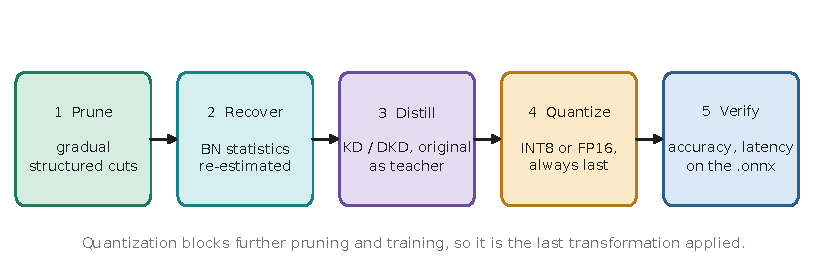
\includegraphics[width=\textwidth]{fig_pipeline.pdf}
\caption{Order of operations in CompressKit. Quantization is applied last because integer weights cannot be pruned or trained further.}
\label{fig:pipeline}
\end{figure}

\section{Project Purpose and Applicability}
The purpose is to make compression a repeatable engineering step with a measurable result instead of a sequence of ad-hoc scripts. The toolkit applies to CNN image classifiers that export to ONNX, on the CPU targets where ONNX Runtime's CPU provider is used: laptops, kiosks, industrial controllers and single-board computers. Typical use is to take a model trained for a specific task, state a budget such as ``at most 0.45 ms median latency and at most 8 points of accuracy loss'', and obtain a file that meets it or a statement that it cannot.

\section{Scope of the Project}
\textbf{In scope.} Classification CNNs with convolution, batch normalisation, residual or plain stacking and a linear classifier head; structured pruning, KD and DKD, INT8 and FP16 post-training quantization, QAT as a fallback; CIFAR-10, a human-action-recognition image dataset, and any image-folder dataset; CPU measurement through ONNX Runtime; a single-notebook workflow on Kaggle and a command-line interface.

\textbf{Out of scope.} Object detection and segmentation models; transformer architectures; GPU or NPU latency; training from scratch beyond the baselines needed to have something to compress. Depthwise-separable networks (MobileNet style) were not exercised and are not claimed.

\section{Organisation of the Report}
Chapter~3 surveys ten related papers and extracts the gaps that motivate the design. Chapter~4 gives the project plan and timeline. Chapter~5 specifies the requirements and datasets. Chapter~6 presents the proposed system: architecture, algorithms and diagrams. Chapter~7 describes the implementation. Chapter~8 reports measured results, verification and the testing. Chapter~9 concludes and lists future work.

% =====================================================================
\chapter{Literature Survey}
\section{Related Work}
Ten papers were studied in detail, spanning pipeline integration, structured pruning, quantization and distillation. For each, the reported claims were checked against the paper's own tables; discrepancies are noted because they shape what the toolkit must verify rather than inherit.

\textbf{Pipeline integration.} Chae and Seo~\cite{chae2026} argue that quantization must be applied last and propose prune, distillation-assisted fine-tuning, quantization-aware training and INT8 export, reusing the uncompressed model as the teacher at two points (compression-aware KD). Results on ResNet-56 and MobileNetV2 are reported in FLOPs and size; GPU hardware is used only for training, and two FLOP tables for the same configuration are inconsistent. Wang et al.~\cite{wang2025} alternate transfer KD and adaptive channel pruning every epoch rather than pruning once. Their headline gains of up to 18.6 points are best-single-task comparisons against the weakest baseline; the aggregate gain over the strongest baseline is 4.4 points, and no latency is measured.

\textbf{Structured pruning.} He et al.'s AMC~\cite{he2018} learns per-layer pruning ratios with a reinforcement-learning agent and reports measured speed-ups of 1.53 times on GPU and 1.95 times on a phone, one of the few papers in the set with on-device latency. The abstract's 2.7-point gain does not reconcile with the paper's own VGG-16 table, where the margin is 0.3 points. Zhou et al.'s AEMC~\cite{zhou2026} identifies an amplitude mismatch when blocks of a residual network are removed and corrects it with a parameter-free rescaling; the aggregate gain hides a per-task collapse on one benchmark, and no latency is reported.

\textbf{Quantization.} Chen et al.~\cite{chen2021} study accuracy against bit width and observe memory reductions of 3.5 to 6.4 times but no speed-up on unmodified CPU or GPU, a direct warning that INT8 file savings do not imply latency savings. VLCQ~\cite{abdelsalam2025} adds variable-length coding to data-free quantization and reaches 12.26 times effective compression at a 3.89-point loss in one best-case configuration, with decoder throughput asserted rather than measured. Khan and Rafat~\cite{khan2025} combine filter pruning with K-means quantization and report 34,052 times compression, but the abstract's accuracies are training accuracies and the test accuracies are 87.39\% and 53.61\%, and the distillation loss described is not the one used in the experiments. Fang et al.~\cite{fang2026} add fake quantization with a straight-through estimator to federated learning; the convergence bounds for the proposed and baseline methods are algebraically identical.

\textbf{Distillation.} Chen et al.~\cite{chen2020} combine feature and noisy-logit distillation with iterative magnitude pruning; the implied compression is 48.4 times rather than the stated 49.5 times, and the claimed speed-up on a Raspberry Pi cannot be attributed to it because the uncompressed teacher did not fit in memory there. Xu et al.'s ReKD~\cite{xu2024} splits logits by rank into head and tail categories and improves on classical KD by 0.6 to 3.7 points, while claiming no extra hyperparameters despite introducing three and reporting no runtime.

\section{Summary of the Surveyed Papers}
\begin{table}[!htbp]
\centering
\small
\begin{tabularx}{\textwidth}{@{}l l X X@{}}
\toprule
Ref. & Topic & Main idea & Gap found on closer reading\\
\midrule
\cite{chae2026} & Pipeline & Prune, KD, QAT, INT8; original model as teacher & FLOPs and size only; inconsistent FLOP tables\\
\cite{wang2025} & Pipeline & Alternate KD and channel pruning each epoch & Best-case gains; no latency\\
\cite{he2018} & Pruning & RL-chosen per-layer ratios & Abstract gain not in own table\\
\cite{zhou2026} & Pruning & Rescale after removing residual blocks & Per-task collapse; no latency\\
\cite{chen2021} & Quantization & Accuracy against bit width & No speed-up without matching hardware\\
\cite{abdelsalam2025} & Quantization & Variable-length coded weights & Best-case ratio; decoder speed unmeasured\\
\cite{khan2025} & Quantization & Pruning plus K-means & Train accuracy in abstract\\
\cite{fang2026} & Quantization & QAT with STE in federated learning & Identical bounds\\
\cite{chen2020} & Distillation & Noisy-logit KD plus pruning & Ratio and Raspberry Pi claims\\
\cite{xu2024} & Distillation & Head and tail category KD & Hidden hyperparameters; no runtime\\
\bottomrule
\end{tabularx}
\caption{Ten surveyed papers and the gap each leaves open.}
\label{tab:survey}
\end{table}

\section{Limitations of Existing Systems}
Three patterns recur across the set. \emph{Proxy substitution}: FLOPs and parameter counts are reported far more consistently than measured on-device latency, and in five of the ten papers hardware mentioned in the text is used only for training. \emph{Best-case reporting}: abstracts quote the best single configuration or the weakest baseline. \emph{Train and test conflation}: the extreme case is~\cite{khan2025}, where the quoted accuracy is the training accuracy.

On the tool side, the common open implementations provide the individual techniques (for example Torch-Pruning for structured pruning~\cite{fang2023} and ONNX Runtime's static quantizer), but not the ordering, the hardware gating, the layer-aware allocation, or the budget search that ties them to a requirement.

\section{Motivation for the Proposed System}
The gaps translate into three evaluation rules that the toolkit enforces: benchmark on the deployment runtime instead of reporting proxies, report what was measured (including the cases where the method loses), and validate every stage on a held-out set rather than on training data. A fourth motivation is practical: a user who has only a latency and accuracy requirement should not have to choose and order the techniques by hand.

% =====================================================================
\chapter{Project Implementation Plan}
\section{Project Schedule}
\subsection{Project Task Set}
The major tasks of the project were:
\begin{itemize}
\item \textbf{Task 1} Study of compression literature and definition of the evaluation rules (Chapter~3).
\item \textbf{Task 2} Core infrastructure: host probe, ONNX export, benchmarking protocol.
\item \textbf{Task 3} Compression stages: structured pruning, BN recalibration, KD and DKD, quantization, QAT, sensitivity analysis.
\item \textbf{Task 4} Orchestration: the staged pipeline, the budget search, the HTML report.
\item \textbf{Task 5} Hardening through edge-case tests and review of silent-failure modes.
\item \textbf{Task 6} Gradual pruning, dataset-agnostic CLI, and the single-notebook Kaggle workflow.
\item \textbf{Task 7} Experiments on ResNet-20, ResNet-56 and VGG-16-BN; verification of the ONNX output; documentation and this report.
\end{itemize}

\subsection{Time Line Chart}
Fig.~\ref{fig:timeline} lays the work out against dates that can be checked in the repository: commit dates (41 commits on six days) and the modification dates of the collected papers, the survey and design documents, the training logs and the draft paper. Bars therefore start with the literature work on 5 September, run through the package split and hardening in mid-September, and continue with the budget-search work on 11 October and the gradual-pruning and Kaggle workflow on 26 and 27 October. No work is recorded between 17 September and 10 October, so that stretch is shown as a hatched break instead of being filled in.

\begin{figure}[H]
\centering
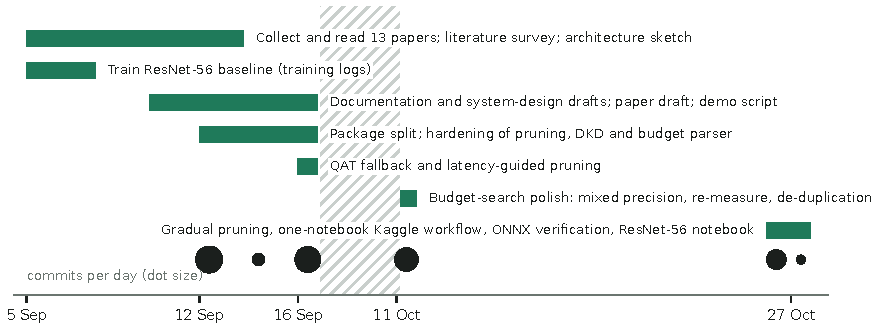
\includegraphics[width=\textwidth]{fig_timeline.pdf}
\caption{Project timeline from commit dates and file modification dates. The hatched band is an axis break (17 September to 10 October, no recorded work). Dots show commits per day.}
\label{fig:timeline}
\end{figure}

% =====================================================================
\chapter{Project Requirement Specification}
\section{Hardware and Software Requirements}
\subsection{Hardware}
Two machines were used, with different roles. The Apple laptop is the deployment-like target on which latency is judged. It also trained the ResNet-20 and ResNet-56 baselines (on its GPU, through Metal) and ran the ResNet-20 compression. The Kaggle notebook ran the full ResNet-56 schedule and VGG-16-BN; the full ResNet-56 run used no GPU, so its fine-tuning ran on the Kaggle CPU.

\begin{table}[!htbp]
\centering
\small
\begin{tabularx}{\textwidth}{@{}c l X X@{}}
\toprule
Sr. & Parameter & Local machine (final timing) & Kaggle notebook\\
\midrule
1 & Processor & Apple M5, 10 logical cores (4 performance) & Intel Xeon, 4 logical cores: 2.20 GHz (ResNet-56) and 2.00 GHz (VGG-16-BN)\\
2 & INT8 support & Fast: i8mm, dotprod, fp16, bf16, neon & Slow (no VNNI): avx2, f16c on the ResNet-56 host; avx2, avx512f, f16c on the VGG-16-BN host\\
3 & Accelerator & Used for training (GPU through Metal); none for timing & ResNet-56: none, CPU only; VGG-16-BN: not recorded\\
4 & Role & Baseline training, ResNet-20 compression, latency and ONNX verification & Full ResNet-56 and VGG-16-BN compression\\
\bottomrule
\end{tabularx}
\caption{Hardware used. The probe results are those recorded by the toolkit's host module.}
\label{tab:hw}
\end{table}

\subsection{Software}
\begin{table}[!htbp]
\centering
\small
\begin{tabular}{@{}l l p{6.5cm}@{}}
\toprule
Component & Version / choice & Purpose\\
\midrule
Python & 3.14.7 (local) & Implementation language\\
PyTorch & 2.14.0 & Model definition, training, fine-tuning\\
Torch-Pruning & DepGraph pruner & Dependency-aware channel removal\\
ONNX Runtime & 1.29.0 & Quantization and all measurements\\
NumPy & 2.5.2 & Array operations, CPU feature flags\\
pytest & configured in \code{pyproject.toml} & 172 tests by default\\
Git and GitHub & -- & Version control and distribution\\
Kaggle Notebook & T4 GPU, internet on & Single end-to-end run environment\\
\bottomrule
\end{tabular}
\caption{Software stack.}
\label{tab:sw}
\end{table}

\section{Functional Requirements}
\begin{enumerate}
\item FR1: Train or load an FP32 classification baseline for CIFAR-10, a human-action-recognition dataset, or any one-folder-per-class image dataset.
\item FR2: Prune a model structurally by a requested ratio, in one or several steps, with per-layer alignment and shared ratios across residual groups.
\item FR3: Re-estimate batch-norm statistics and fine-tune with KD or DKD against the original model as teacher.
\item FR4: Quantize to INT8 or FP16 through ONNX Runtime, with an automatic choice gated by the host, and fall back to QAT when asked.
\item FR5: Rank layers by quantization sensitivity and use the ranking for exclusions and pruning ratios.
\item FR6: Accept a budget (latency, accuracy drop, minimum accuracy, size) and search for the cheapest configuration meeting it.
\item FR7: Benchmark every stage on the exported ONNX file and write \code{results.json}, an HTML report and the \code{.onnx} file.
\item FR8: Verify the compressed file against the original on real test images.
\end{enumerate}

\section{Non-Functional Requirements}
\begin{itemize}
\item \textbf{Measurement integrity.} Latency uses one ONNX Runtime session configuration for every precision: one thread, batch size 1, 50 warm-up runs, 200 timed runs, median and 95th percentile reported. Accuracy is measured on the exported file.
\item \textbf{No leakage.} BN re-estimation and quantization calibration read only the training split.
\item \textbf{Reproducibility.} The train/test split of folder datasets is deterministic by sorted file name; random seeds are fixed for calibration subsets.
\item \textbf{Honest failure.} Unmet budgets return the best trade-off and say so. Operators without an INT8 kernel are counted in the report.
\item \textbf{Usability.} One command or one notebook run produces all outputs.
\item \textbf{Portability.} Pure Python, CPU inference, no vendor-specific runtime.
\end{itemize}

\section{Dataset Description}
\begin{description}
\item[CIFAR-10~\cite{krizhevsky2009}] 60,000 colour images of $32\times32$ pixels in 10 classes: 50,000 for training and 10,000 for testing. Used for ResNet-20, ResNet-56 and VGG-16-BN. Input shape for the toolkit: $1\times3\times32\times32$.
\item[Human Action Recognition (HAR)] A 15-class image dataset at $224\times224$ input, read through a loader that finds the data under the Kaggle input directory. The ResNet-18 baseline path is implemented; its Kaggle run was not completed within this project, so no HAR accuracy is claimed.
\item[Image folder] Any dataset with one sub-directory per class. A fixed 15\% of each class, taken from the end of the sorted file list, is held out as the test set.
\end{description}

% =====================================================================
\chapter{Proposed System}
\section{Overall System Architecture}
Fig.~\ref{fig:system} shows the whole system from what the user supplies to what it delivers. Three inputs go in: a trained FP32 checkpoint, a dataset with train, test and calibration views, and a request, which is either a fixed recipe (prune ratio, steps, fine-tune epochs, precision) or a budget string. The toolkit itself has five cooperating parts. An \emph{entry point} (command line, Python API or notebook) builds a \code{Pipeline}. The \emph{host probe} reads the CPU's instruction-set features and decides whether INT8 is allowed. The \emph{pipeline controller} checks the stage order and runs a pre-flight summary. The \emph{stages} transform the model in a fixed order. The \emph{search layer} sits beside them and, for a budget request, decides which stages to use. After every stage the \emph{measurement} component exports the model to ONNX and measures it in ONNX Runtime, and the \emph{reporting} component turns all measurements into the three outputs: the compressed \code{.onnx}, an HTML report and \code{results.json}. Finally the delivered file is re-measured on the target host and compared with the original.

\begin{figure}[H]
\centering
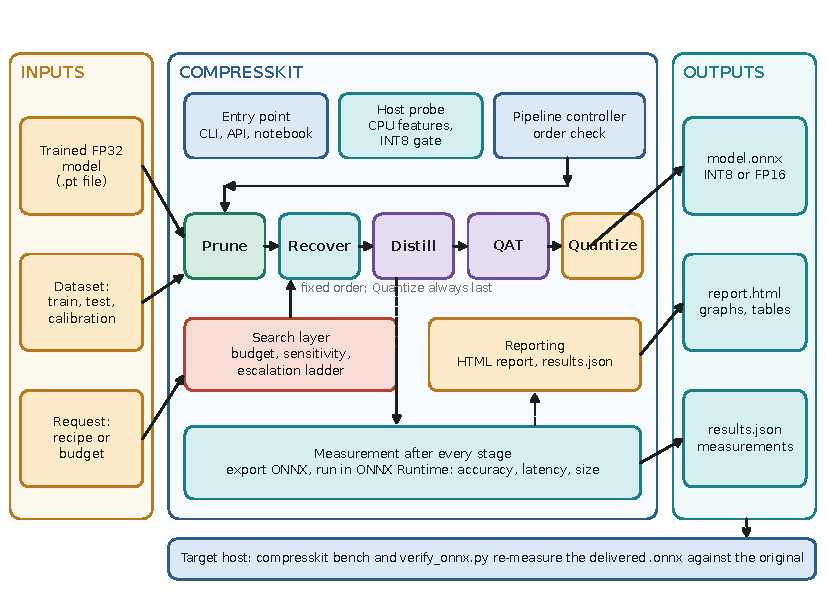
\includegraphics[width=0.9\textwidth]{fig_system.pdf}
\caption{Overall system architecture of CompressKit: inputs, the toolkit with its stages, search, measurement and reporting, and the three outputs.}
\label{fig:system}
\end{figure}

\section{Layered Architecture and Modules}
Seen as a code base, CompressKit is a small library with three entry points, four compression stages, an orchestration layer and a shared core (Fig.~\ref{fig:arch}). The core is cross-cutting: the host probe attaches the machine's capabilities to every measurement, the benchmark module produces the numbers all stages are judged by, and the export module writes ONNX.

\begin{figure}[H]
\centering
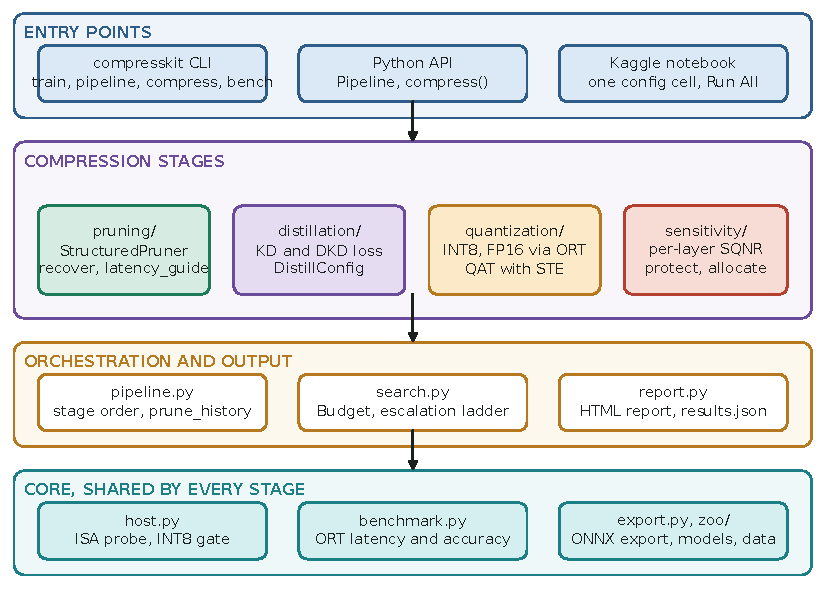
\includegraphics[width=0.66\textwidth]{fig_architecture.pdf}
\caption{Layered architecture of CompressKit. Directory names match the source tree.}
\label{fig:arch}
\end{figure}

\subsection{Modules}
\textbf{Host probe} (\code{core/host.py}). Reads the CPU's instruction-set features. INT8 is recommended only when at least one of AMX-INT8, AVX-512 VNNI, AVX-VNNI, I8MM or DotProd is present, because without a fused integer dot-product INT8 is routinely slower than FP32 while still producing a smaller file. Otherwise FP16 is the default and INT8 becomes an explicit, warned opt-in. The probe result is stored with each measurement.

\textbf{Structured pruner} (\code{pruning/prune.py}). Wraps Torch-Pruning's dependency graph~\cite{fang2023}. It never prunes the classifier, always works on a deep copy of the model, and adds three behaviours described next: per-layer SIMD alignment, shared ratios across residual groups, and gradual steps.

\textbf{Recovery} (\code{pruning/recover.py}). Resets batch-norm running statistics and recomputes them as a cumulative average over training batches, so the stale statistics of the old network are not applied to the new one.

\textbf{Distillation} (\code{distillation/distill.py}). KD and decoupled KD with the original, uncompressed model as teacher, so no second network has to be trained~\cite{chae2026}.

\textbf{Quantization} (\code{quantization/}). Static post-training quantization through ONNX Runtime with per-channel weights, calibrated on a subset of the training split, plus an operator-coverage audit; QAT with a straight-through estimator~\cite{bengio2013} as a fallback.

\textbf{Sensitivity} (\code{sensitivity/analysis.py}). Label-free per-layer ranking used for exclusions and non-uniform pruning ratios.

\textbf{Pipeline, search and report} (\code{pipeline.py}, \code{search.py}, \code{report.py}). Stage orchestration, the budget search, and the HTML and JSON output.

\section{The Compression Pipeline in Detail}
\subsection{Stage Model and Ordering Rule}
The pipeline is a chainable builder: \code{Pipeline(model, calibration, test, train)} followed by calls such as \code{.prune(0.5, steps=3, fine\_tune\_epochs=2).recover().quantize()} only \emph{records} the stages. Nothing runs until \code{run()}. Two copies of the model are made at construction. One is the untouched \emph{original}, which is both the accuracy reference and the distillation teacher, so it has to survive every in-place stage; the other is the working model.

One rule is enforced before any compute is spent: \code{quantize} must be the last stage, otherwise \code{run()} raises an error. Integer weights cannot be pruned structurally and cannot be trained further, so any stage placed after quantization would either fail or silently undo it~\cite{chae2026}. A \code{preflight()} call prints the host capabilities, parameter count, calibration size, the protected classifier layer and the planned stage list, and warns if quantize is not last.

\subsection{Stage by Stage}
Fig.~\ref{fig:pipedetail} gives the data path and Table~\ref{tab:stages} summarises what each stage takes, does and records.

\begin{figure}[H]
\centering
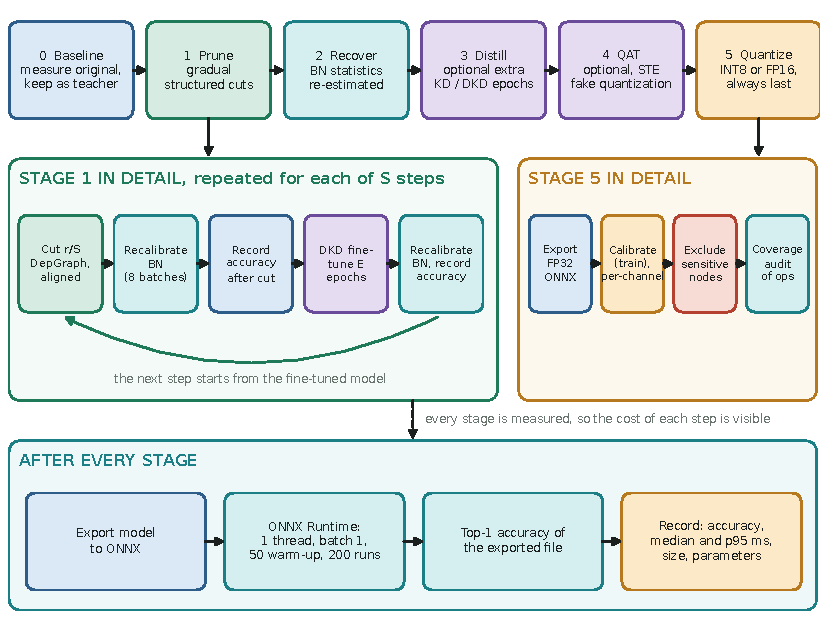
\includegraphics[width=0.9\textwidth]{fig_pipeline_detail.pdf}
\caption{The pipeline in detail: the six stages, the pruning loop and the quantization steps expanded, and the measurement performed after every stage.}
\label{fig:pipedetail}
\end{figure}

\begin{table}[!htbp]
\centering
\small
\setlength{\tabcolsep}{3pt}
\begin{tabularx}{\textwidth}{@{}l X X X@{}}
\toprule
Stage & What it does & Needs & Guard or record\\
\midrule
0 Baseline & Exports the original to ONNX and measures it & Test split & Teacher and reference for all later stages\\
1 Prune & $S$ cuts of $r/S$ of the channels, each followed by BN recalibration and DKD fine-tuning & Calibration and train loaders & Classifier never pruned; works on a deep copy; \code{prune\_history} rows\\
2 Recover & Resets BN running statistics and recomputes them as a cumulative average & Calibration loader (train split) & No labels, no back-propagation\\
3 Distill & Extra KD or DKD epochs against the original & Train loader & Error if no training data is given\\
4 QAT & Fake quantization with a straight-through estimator & Train loader & Fallback when post-training INT8 misses accuracy\\
5 Quantize & Exports FP32 ONNX, calibrates, writes INT8 or FP16 & Calibration loader, host probe & Sensitive layers excluded; operator coverage audited; must be last\\
\bottomrule
\end{tabularx}
\caption{Pipeline stages with inputs and guards.}
\label{tab:stages}
\end{table}

\textbf{Pruning loop.} Each of the $S$ steps cuts a fraction of the channels, recalibrates the batch-norm statistics on eight calibration batches, records the accuracy right after the cut, fine-tunes for $E$ epochs with decoupled KD against the original, recalibrates again and records the accuracy after the fine-tune. Recalibrating between steps matters: the next importance ranking would otherwise be computed on a mis-normalised network. The last cut has no step after it, so it receives the same cut, fine-tune, recalibrate treatment explicitly. This is the code path where the defect described in Section~\ref{sec:defect} was found: the pruner works on its own deep copy, so the final fine-tune must act on the pruner's model and not on the caller's still-unpruned variable.

\textbf{Recover and distill.} Recovery needs no labels and costs a few forward passes. Distillation spends epochs of training and is used when fine-tuning inside the pruning loop is not enough.

\textbf{Quantize.} The working model is exported to an FP32 ONNX file; layer names from the sensitivity ranking are mapped to node names in \emph{that} exported graph; ONNX Runtime's static quantizer calibrates on the training subset with per-channel weight scales; and the result is audited for how many compute operators actually received an INT8 kernel. If the host probe reports no fused integer instructions, the default precision is FP16 and INT8 requires an explicit opt-in.

\textbf{Measurement.} After every stage the model is exported and measured under the same protocol. A stage's cost is therefore visible, and a stage that did not help (such as recovery after fine-tuning, in Chapter~8) shows as a flat step instead of being assumed useful.

\subsection{The Run Procedure}
\begin{algorithm}[H]
\caption{\code{Pipeline.run}}\label{alg:run}
\KwIn{ordered stages $T_1\dots T_n$, original model $M_0$, loaders}
\KwOut{list of measurements, prune history, warnings}
\lIf{quantize appears and is not last}{raise error}
baseline $\gets$ \textsc{Measure}($M_0$); $M \gets \mathrm{copy}(M_0)$\;
\For{$i \gets 1$ \KwTo $n$}{
  \Switch{kind of $T_i$}{
    \Case{prune}{ run Algorithm~\ref{alg:gradual} on $M$; $M \gets$ pruner's model }
    \Case{recover}{ recalibrate BN of $M$ on calibration batches }
    \Case{distill}{ distill $M$ from $M_0$ }
    \Case{qat}{ fake-quantize and fine-tune $M$ }
    \Case{quantize}{ export $M$; calibrate; write INT8 or FP16; audit coverage }
  }
  append \textsc{Measure}(result of $T_i$) to the list\;
}
\Return measurements, history, warnings\;
\end{algorithm}

\subsection{Why This Order}
Pruning first, because it changes the architecture and everything after must fit the smaller network. Batch-norm recalibration and distillation next, because they repair the accuracy lost by the cut while all weights are still float and trainable. Quantization last, because converting weights to integers is hard to reverse and blocks further training. The same order is used by the budget search, which differs only in \emph{how many} of these stages it applies.

\subsection{Two Ways to Drive the Pipeline}
In \emph{fixed-recipe mode} the user states the stages and their parameters, for example \code{compresskit pipeline --prune 0.5 --steps 3 --fine-tune-epochs 2}. In \emph{budget mode} the search layer builds one pipeline per ladder rung (Section~\ref{sec:budget}), runs it, compares the measurements with the budget and escalates only if the budget is unmet. Both modes call the same \code{Pipeline.run}, so every number in a report was produced by the same code path.

\section{Core Algorithms}
\subsection{Pruning: Residual Groups and Alignment}
In a residual network the output channels of a convolution may be summed with a shortcut, so several layers must keep exactly the same channel indices. Torch-Pruning exposes these as dependency groups. In ResNet-20, 12 groups tie two or more layers: three stage-wide groups of eight layers each, and nine groups that pair a convolution with its batch norm. If two layers in one group request different ratios the pruner would pick one arbitrarily. CompressKit resolves each group toward its most protective member, that is, the lowest requested ratio.


Channel counts are rounded to multiples of a SIMD-friendly alignment (8, 16 or 32). A single global alignment fails for narrow layers: Torch-Pruning floors the kept count to a multiple of the alignment, a layer whose width is under two alignment blocks floors to zero, the group is rejected as invalid, and the layer silently keeps every channel. The toolkit instead computes the nearest achievable aligned count per layer and halves the alignment only for the layer that needs it (Algorithm~\ref{alg:align}, Fig.~\ref{fig:align}).

\begin{algorithm}[H]
\caption{Per-layer aligned ratio (from \code{\_aligned\_ratio})}\label{alg:align}
\KwIn{layer width $w$, requested ratio $r$, alignment $a$}
\KwOut{effective ratio $r'$, alignment used $a'$}
$a' \gets a$\;
\While{$a' > 1$ \textbf{and} $\lfloor w / a' \rfloor < 2$}{$a' \gets \lfloor a'/2 \rfloor$}
\If{$a' \le 1$}{ $k \gets \max(1, \mathrm{round}(w(1-r)))$; \Return $(1-k/w,\ a')$ }
$n \gets \min\big(\lfloor w/a' \rfloor,\ \max(1,\ \mathrm{round}(w(1-r)/a'))\big)$\;
$k \gets n\,a'$; \Return $(1-k/w,\ a')$\;
\end{algorithm}

For example, a 64-channel layer at requested ratio 0.7 keeps 16 channels with alignment 16 (effective ratio 0.75) and 32 channels with alignment 32 (effective ratio 0.5): the result is the nearest multiple, not the floor. A 16-channel layer at ratio 0.5 keeps 8, and an 8-channel layer keeps 4 by relaxing the alignment to 4. These values come from a 180-case table generated by the real function, which is kept as a golden test of the alignment rule.

\begin{figure}[H]
\centering
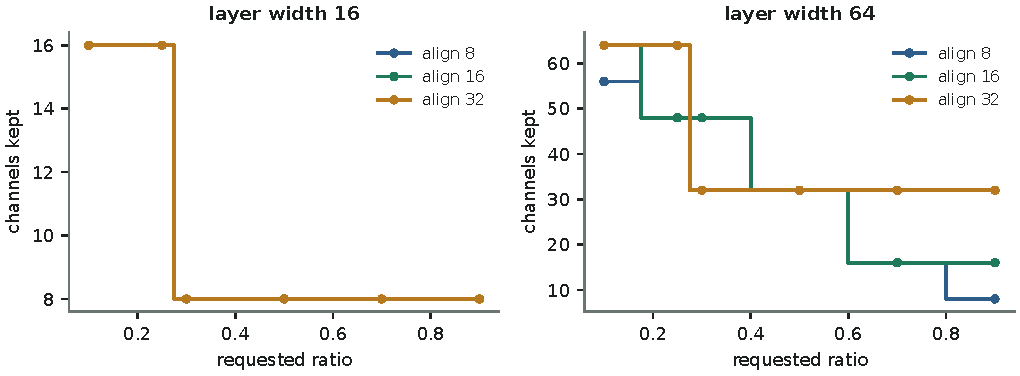
\includegraphics[width=0.8\textwidth]{fig_align.pdf}
\caption{Channels kept against requested ratio for a layer of width 16 (left) and 64 (right) under alignments 8, 16 and 32, computed by the toolkit's \code{\_aligned\_ratio}. A narrow layer cannot satisfy a large alignment, so all curves coincide on the left.}
\label{fig:align}
\end{figure}

\subsection{Gradual Pruning with Fine-Tuning}
Instead of removing all channels at once, the pruner removes them in $S$ equal steps and fine-tunes after each (Algorithm~\ref{alg:gradual}). The motivation is that a smaller cut is easier to recover from~\cite{wang2025}; whether this beats one-shot pruning at an equal fine-tuning budget is tested in Chapter~8. Every step is recorded as the accuracy right after the cut and right after the fine-tune.

\begin{algorithm}[H]
\caption{Gradual structured pruning with interleaved distillation}\label{alg:gradual}
\KwIn{trained model $M_0$ (teacher), ratio $r$, steps $S$, epochs per step $E$}
\KwOut{pruned model $M_S$, history of (acc. after cut, acc. after fine-tune)}
$P \gets \textsc{StructuredPruner}(\mathrm{copy}(M_0), r, S)$\;
\For{$s \gets 1$ \KwTo $S$}{
  $M \gets P.\mathrm{step}()$ \tcp*{remove $r/S$ of the way}
  record accuracy of $M$; recalibrate BN statistics on train batches\;
  \If{$E > 0$}{ fine-tune $M$ for $E$ epochs with DKD against $M_0$; record accuracy }
}
\Return $M$ (the pruner's own model, not the original)\;
\end{algorithm}

\subsection{Distillation Loss}
With student logits $z_s$, teacher logits $z_t$, temperature $T$ and target class $c$, decoupled KD~\cite{zhao2022} is
\begin{equation}
\mathcal{L}_{\mathrm{DKD}} = \alpha\, \mathrm{TCKD} + \beta\, \mathrm{NCKD},
\end{equation}
where TCKD is the KL divergence between the two-way distributions $(p_c,\,1-p_c)$ of teacher and student, and NCKD is the KL divergence between the teacher and student distributions over the non-target classes after masking the target before the softmax. Both terms are scaled by $T^2$. Defaults are $T=4$, $\alpha=1$ and $\beta=8$; plain KD uses $\alpha=0.3$. The final loss adds the cross-entropy on the labels. The target probability is clamped away from 0 and 1 so that a confident student cannot produce $\log 0$ and a NaN loss.

\subsection{Quantization and Sensitivity}
Weight quantization maps a tensor to 8-bit integers with a scale per output channel. The sensitivity of a layer is measured without labels: its weights alone are replaced by their INT8 quantize--dequantize round trip, and the signal-to-quantization-noise ratio at the output logits is computed,
\begin{equation}
\mathrm{SQNR}_\ell = 10\log_{10}\frac{\lVert y\rVert^2}{\lVert y-\hat{y}_\ell\rVert^2}\ \text{dB},
\end{equation}
where $\hat{y}_\ell$ are the logits with layer $\ell$ perturbed. For $L$ layers this takes $L+1$ forward passes. A low SQNR marks a layer that quantization hurts. The same ranking supplies the layers kept in FP32 and the layers that receive a smaller pruning ratio, which gives a non-uniform allocation without the reinforcement-learning search of~\cite{he2018}.

\subsection{Budget Search}\label{sec:budget}
A budget is a string such as \code{latency<0.45ms,accuracy\_drop<8\%}. \code{Budget.parse} turns it into limits on latency, accuracy drop, minimum accuracy and size. The search tries the cheapest rung first and moves on only if the budget is unmet (Fig.~\ref{fig:ladder}); borderline passes are re-measured at full fidelity before being trusted, and prune trials that resolve to an already measured architecture are skipped.

\begin{figure}[!htbp]
\centering
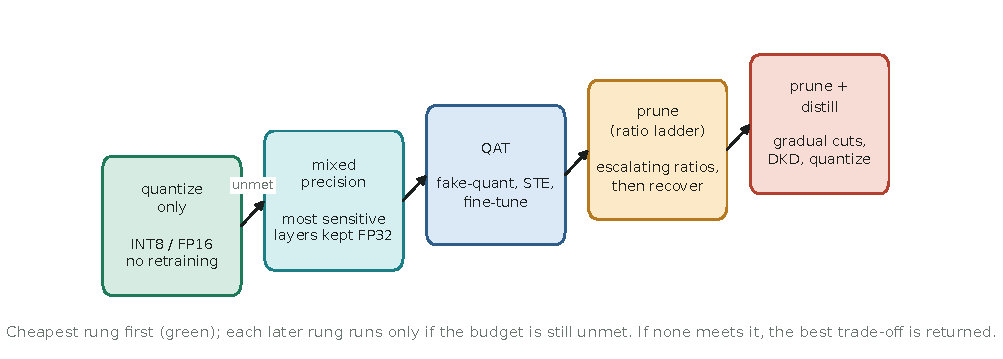
\includegraphics[width=0.88\textwidth]{fig_ladder.pdf}
\caption{Escalation ladder of the budget search. Colours distinguish the rungs; the cheapest is on the left.}
\label{fig:ladder}
\end{figure}

\section{Data Flow Diagrams}
\subsection{DFD Level 0}
\begin{figure}[H]
\centering
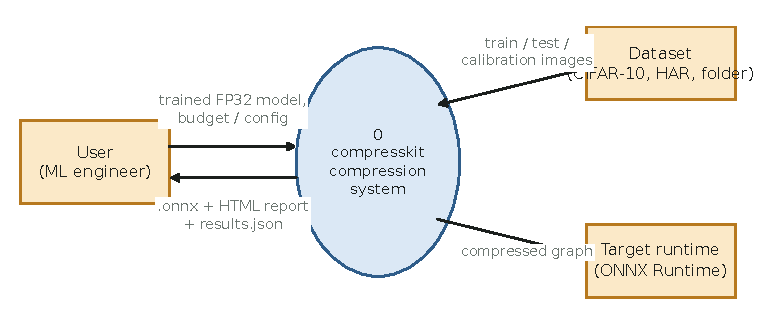
\includegraphics[width=0.62\textwidth]{fig_dfd0.pdf}
\caption{Data flow diagram, level 0: the toolkit as one process between the user, the dataset and the target runtime.}
\label{fig:dfd0}
\end{figure}

\subsection{DFD Level 1}
\begin{figure}[H]
\centering
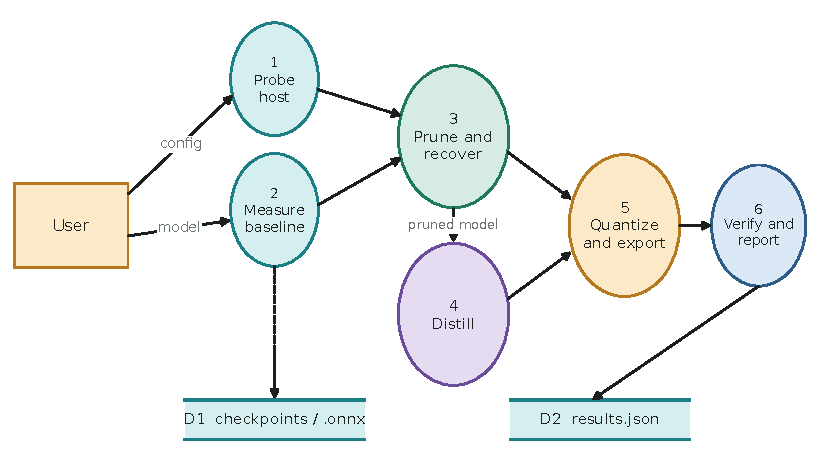
\includegraphics[width=0.86\textwidth]{fig_dfd1.pdf}
\caption{Data flow diagram, level 1: the six processes of one compression run.}
\label{fig:dfd1}
\end{figure}

\subsection{DFD Level 2}
Level 2 expands process 3 (prune and recover).
\begin{figure}[H]
\centering
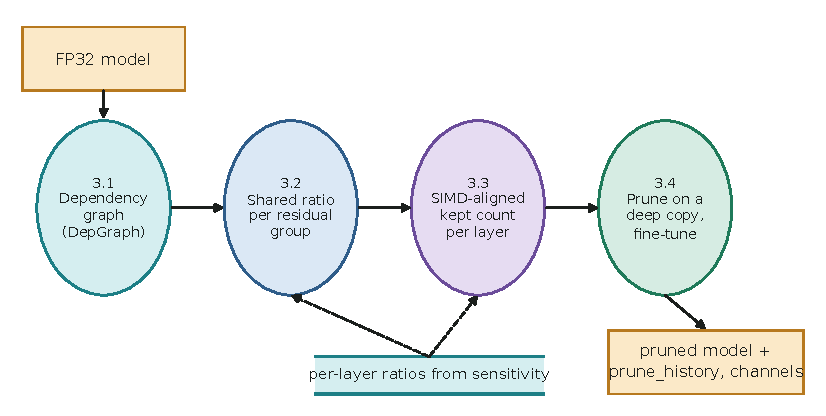
\includegraphics[width=0.86\textwidth]{fig_dfd2.pdf}
\caption{Data flow diagram, level 2: the pruning process.}
\label{fig:dfd2}
\end{figure}

\section{UML Diagrams}
\subsection{Use Case Diagram}
\begin{figure}[H]
\centering
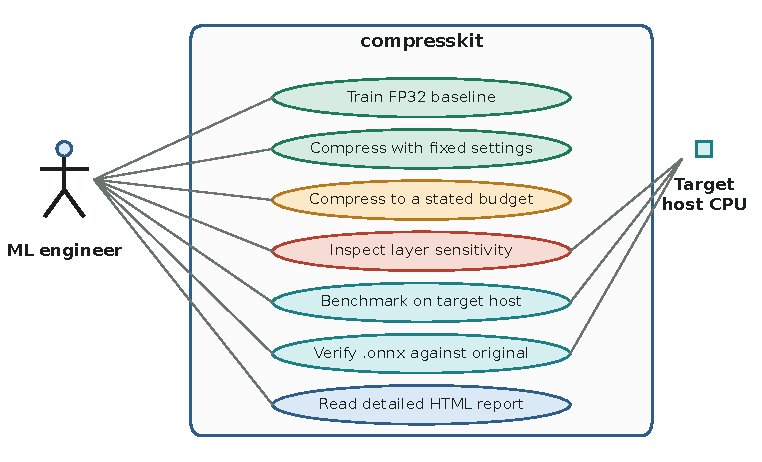
\includegraphics[width=0.6\textwidth]{fig_usecase.pdf}
\caption{Use case diagram. The target host CPU is the secondary actor because latency and INT8 support are properties of that machine.}
\label{fig:usecase}
\end{figure}

\subsection{Sequence Diagram}
\begin{figure}[H]
\centering
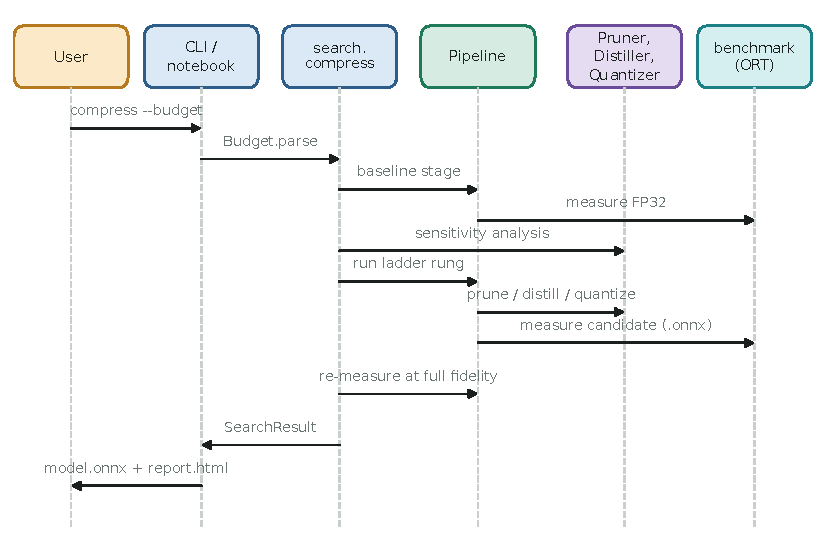
\includegraphics[width=0.88\textwidth]{fig_sequence.pdf}
\caption{Sequence of a budget-driven \code{compress} run.}
\label{fig:sequence}
\end{figure}

\subsection{Class Diagram}
The classes below are the main data carriers; each is a Python dataclass or a small class in the named module, and the field names are those in the source.
\begin{figure}[H]
\centering
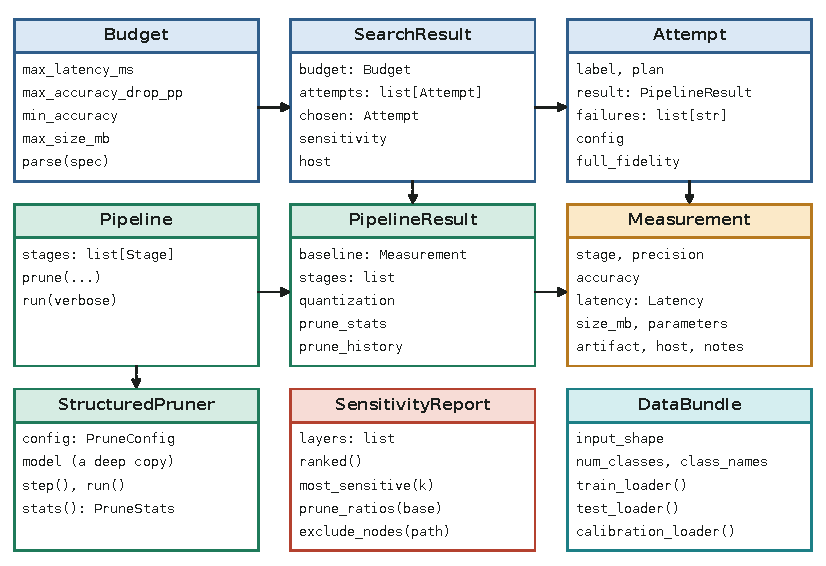
\includegraphics[width=0.88\textwidth]{fig_classes.pdf}
\caption{Class diagram of the principal types.}
\label{fig:classes}
\end{figure}

% =====================================================================
\chapter{System Implementation}
\section{Package Layout}
The package has 26 Python modules and 5,054 lines of source. The split into subpackages follows the stages, so a user can import the pruner without pulling in the quantizer. Project-specific code (the example networks and dataset loaders) lives in \code{zoo/} and is not part of the core API.

The largest modules are \code{search.py} (638 lines), \code{pruning/prune.py} (530), \code{report.py} (435), \code{pipeline.py} (420), \code{core/benchmark.py} (352) and \code{quantization/quantize.py} (338); the CLI is 329 lines and the example models, datasets and training code in \code{zoo/} about 700.

\section{Command-Line Interface}
The same flow is available from the command line. A complete run on CIFAR-10 is two commands:
\begin{lstlisting}[language=bash]
compresskit train --arch resnet20
compresskit pipeline --model checkpoints/resnet20_fp32.pt \
    --prune 0.5 --steps 3 --fine-tune-epochs 2 --loss dkd \
    --precision auto --report report.html
\end{lstlisting}
To compress to a requirement instead of a fixed recipe:
\begin{lstlisting}[language=bash]
compresskit compress --model checkpoints/resnet20_fp32.pt \
    --budget "latency<0.45ms,accuracy_drop<8%" --report report.html
\end{lstlisting}
Deployment latency on the target is re-measured with \code{compresskit bench model.onnx}, and the compressed file is compared with the original on real test images by the verification script \code{verify\_onnx.py}.

\section{Selected Code}
The per-layer alignment rule of Algorithm~\ref{alg:align}, as implemented:
\begin{lstlisting}[language=Python]
def _aligned_ratio(width, ratio, align):
    layer_align = align if align and align > 1 else 1
    while layer_align > 1 and width // layer_align < 2:
        layer_align //= 2
    if layer_align <= 1:
        kept = max(1, min(width, round(width * (1 - ratio))))
        return 1 - kept / width, layer_align
    desired_kept = width * (1 - ratio)
    max_blocks = width // layer_align
    n_blocks = min(max_blocks, max(1, round(desired_kept / layer_align)))
    kept = n_blocks * layer_align
    return 1 - kept / width, layer_align
\end{lstlisting}
The decoupled KD loss, including the numerical guard:
\begin{lstlisting}[language=Python]
def binary(prob):
    target_p = prob[target_mask].unsqueeze(1).clamp(min=1e-7, max=1.0 - 1e-7)
    return torch.cat([target_p, 1.0 - target_p], dim=1)

tckd = F.kl_div(binary(student_prob).log(), binary(teacher_prob),
                reduction="batchmean") * (temperature ** 2)
masked_student = student_logits / temperature - 1000.0 * target_mask
masked_teacher = teacher_logits / temperature - 1000.0 * target_mask
# nckd: KL between the renormalised non-target distributions, scaled by T**2
return alpha * tckd + beta * nckd
\end{lstlisting}

\section{One-Notebook Workflow}
The project fixed one working environment. Code lives on GitHub; one Kaggle notebook (\code{kaggle/compresskit\_end\_to\_end.ipynb}) does setup, data, training, compression, ONNX evaluation and report generation under \emph{Run All}, driven by one configuration cell (model, mode manual or budget, prune ratio, steps, fine-tune epochs, loss, precision). Models are not copied between machines while the work runs; the output folder is downloaded once at the end and the final latency check runs on the local machine. Because the Kaggle CPU has no fast INT8, the notebook forces INT8 when asked and the report states that its latency is not the target's.

\section{A Defect Found by Verification}\label{sec:defect}
The first end-to-end ResNet-20 run printed 88\% accuracy in its log, but loading the exported \code{.onnx} and testing it on real images gave 47\%. The cause was in the pipeline: the pruner operates on a deep copy of the model, and the final fine-tune step was applied to the original, unpruned model, while the exported graph came from the pruner's copy. The fix is one line, fine-tuning \code{pruner.model} instead of the caller's variable, and a regression test (\code{test\_every\_fine\_tune\_step\_acts\_on\_the\_pruned\_model}) was written first, shown to fail on the old code and to pass after the change. This is why accuracy is measured on the exported file and not on the in-memory model.

% =====================================================================
\chapter{Results and Testing}
All numbers in this chapter were produced by the toolkit. Where a result is not from a full, final run, it is labelled.

\section{Experimental Setup}
Three CIFAR-10 networks were compressed with a requested channel ratio of 0.5, DKD fine-tuning, and INT8 quantization last. Table~\ref{tab:setup} states the schedule and where each was run.

\begin{table}[!htbp]
\centering
\small
\begin{tabularx}{\textwidth}{@{}l l l X@{}}
\toprule
Model & Schedule & Run on & Status\\
\midrule
ResNet-20 & 3 $\times$ 2 DKD epochs & Apple M5 (INT8 fast) & Measured\\
ResNet-56 (smoke) & 2 $\times$ 1 DKD epoch & Apple M5 & Short smoke run\\
ResNet-56 (full) & 5 $\times$ 5 DKD epochs & Kaggle Xeon CPU & Transcribed from the notebook log; Kaggle-CPU latency\\
VGG-16-BN & 5 $\times$ 5 DKD epochs & Kaggle Xeon CPU & Transcribed from the Kaggle log; Kaggle-CPU latency\\
\bottomrule
\end{tabularx}
\caption{Experimental runs and their status.}
\label{tab:setup}
\end{table}

\section{Protocol}
\textbf{Baselines.} The ResNet-20 and ResNet-56 baselines were trained from scratch for 60 epochs on the full 50,000 training images, with SGD (Nesterov momentum 0.9, weight decay $5\times10^{-4}$), a peak learning rate of 0.1, one warm-up epoch followed by a cosine decay, and random-crop (padding 4) and horizontal-flip augmentation. The seed was not recorded, and the VGG-16-BN baseline recipe is not recorded in the repository.

\textbf{Fine-tuning.} Each pruning step is followed by DKD fine-tuning with SGD (momentum), a learning rate of 0.005 with warm-up and cosine decay, temperature 4, $\alpha=1$ and $\beta=8$. ``2 DKD epochs per step'' means two full passes over the 50,000 training images after each cut, so the three-step ResNet-20 run uses six passes in total. The unpruned FP32 baseline is the teacher.

\textbf{Channel selection.} Channels are ranked by the group L1 norm of their weights across each dependency group (Torch-Pruning's group magnitude importance), the only criterion used in any reported run. The headline runs use one uniform ratio for every layer and no per-layer overrides; per-layer overrides from the sensitivity ranking appear only in the budget search (Section~\ref{sec:search}).

\textbf{Quantization and timing.} INT8 uses ONNX Runtime static quantization in QDQ format: per-channel symmetric INT8 weights, asymmetric activations (signed on Arm, unsigned on x86), MinMax calibration on 512 training images, and 7-bit range reduction only on x86 hosts without VNNI. Every latency is the median of 200 timed runs after 50 warm-up runs, at batch size 1 on one thread, with the CPU execution provider and full graph optimization. FP16 export exists but was not run in any experiment reported here.

\textbf{Splits.} Accuracy in every table is measured on the 10,000 CIFAR-10 test images. Sensitivity and batch-norm re-estimation use training images only. The budget search of Section~\ref{sec:search} originally ranked candidates on the test set; it was re-run with a held-out validation split to remove that bias.

\section{Compression Results}
\begin{table}[!htbp]
\centering
\small
\setlength{\tabcolsep}{4pt}
\begin{tabular}{@{}l l r r r r@{}}
\toprule
Model & Stage & Acc. (\%) & Size (MB) & Latency (ms) & Parameters\\
\midrule
\multirow{4}{*}{ResNet-20} & FP32 baseline & 91.54 & 1.046 & 1.452 & 272,474\\
 & pruned & 83.97 & 0.270 & 0.649 & 68,786\\
 & pruned and recovered & 83.97 & 0.270 & 0.671 & 68,786\\
 & INT8 & 84.00 & 0.115 & 0.460 & 68,786\\
\midrule
\multirow{4}{*}{ResNet-56} & FP32 baseline & 93.18 & 3.281 & 2.729 & 855,770\\
 & pruned & 81.73 & 0.842 & 0.936 & 215,282\\
 & pruned and recovered & 81.73 & 0.842 & 1.027 & 215,282\\
 & INT8 & 81.91 & 0.335 & 0.664 & 215,282\\
\midrule
\multirow{4}{*}{VGG-16-BN} & FP32 baseline & 93.20 & 56.16 & 9.042 & 14,724,042\\
 & pruned & 90.25 & 14.05 & 1.995 & 3,684,842\\
 & pruned and recovered & 90.25 & 14.05 & 1.859 & 3,684,842\\
 & INT8 & 90.18 & 3.57 & 1.133 & 3,684,842\\
\bottomrule
\end{tabular}
\caption[Per-stage measurements for the three models.]{Per-stage measurements. ResNet-20 and ResNet-56 on Apple M5; ResNet-56 is the short smoke schedule; VGG-16-BN on a Kaggle CPU, transcribed from the run log.}
\label{tab:results}
\end{table}

\begin{table}[!htbp]
\centering
\small
\setlength{\tabcolsep}{4pt}
\begin{tabular}{@{}l r r r r@{}}
\toprule
Model & Size red. & Speed-up & Acc. cost (pp) & MACs (M)\\
\midrule
ResNet-20 & 9.11$\times$ & 3.16$\times$ & 7.54 & 41.2 to 10.5\\
ResNet-56 (smoke) & 9.79$\times$ & 4.11$\times$ & 11.27 & 126.8 to 32.1\\
VGG-16-BN (Kaggle CPU) & 15.72$\times$ & 7.98$\times$ & 3.02 & 314.2 to 79.2\\
\bottomrule
\end{tabular}
\caption[Compression ratios beside their accuracy cost.]{Compression ratios, each beside the accuracy it cost. The VGG-16-BN speed-up is on a CPU without fast INT8 and is not a deployment figure.}
\label{tab:ratios}
\end{table}

\begin{table}[!htbp]
\centering
\small
\begin{tabular}{@{}l r r r r@{}}
\toprule
Stage & Acc. (\%) & Size (MB) & Latency (ms) & Parameters\\
\midrule
FP32 baseline & 93.18 & 3.28 & 4.655 & 855,770\\
pruned and recovered & 89.20 & 0.84 & 1.649 & 215,282\\
INT8 & 89.28 & 0.33 & 2.030 & 215,282\\
\bottomrule
\end{tabular}
\caption[ResNet-56, full schedule, Kaggle CPU (transcribed).]{ResNet-56, full schedule (5 steps of 5 DKD epochs, requested ratio 0.5), run on a Kaggle Xeon CPU and transcribed from the notebook log. Parameters fall 3.98 times, MACs from 126.8 M to 32.1 M, the file is 9.81 times smaller, and accuracy falls 3.90 points. On this host the INT8 file is slower (2.030 ms) than the pruned FP32 one (1.617 ms), because the CPU has no fused integer instructions.}
\label{tab:r56full}
\end{table}

Checked on 2,000 real test images, the original ResNet-56 scored 93.05\% and the compressed file 89.90\%, and the two agreed on 91.65\% of them. Accuracy after each cut and after its fine-tune was 83.35 $\to$ 90.19, 83.84 $\to$ 89.68, 82.15 $\to$ 88.95, 76.31 $\to$ 88.59 and 64.56 $\to$ 89.20 per cent. The final cut is the hardest: accuracy falls to 64.56\% and fine-tuning restores it to 89.20\%, which is why the last step must act on the pruned network (Section~\ref{sec:defect}).

\begin{figure}[!htbp]
\centering
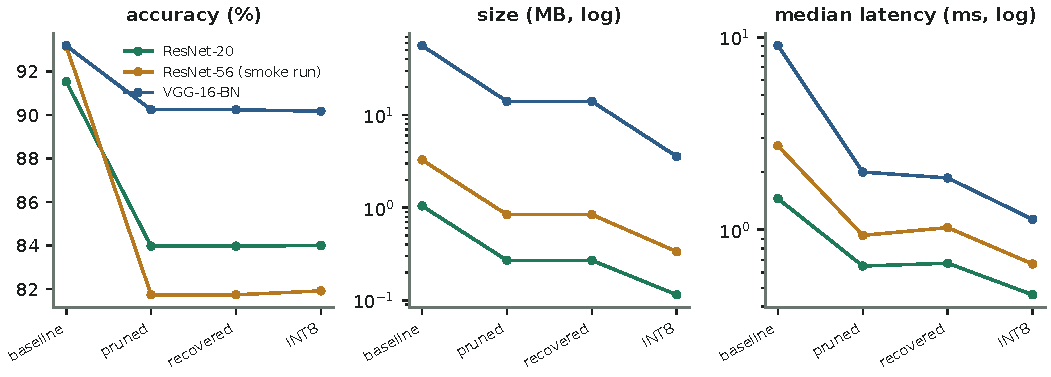
\includegraphics[width=0.74\textwidth]{fig_stages.pdf}
\caption{Accuracy, size and median latency through the four stages for the three recorded runs (size and latency on log axes).}
\label{fig:stages}
\end{figure}


Three observations follow. First, quantization alone moved accuracy by at most 0.18 points in these runs (ResNet-20 83.97 to 84.00, ResNet-56 81.73 to 81.91, VGG-16-BN 90.25 to 90.18), so almost all of the accuracy cost belongs to pruning. Second, the pruned FP32 model is already about twice as fast as the baseline on ResNet-20 (1.452 to 0.649 ms); INT8 on a host with fused kernels adds a further drop to 0.460 ms. Third, the recovery stage by itself changed nothing visible once fine-tuning had been done, because the fine-tune had already re-estimated the statistics; its effect is isolated below.

\section{Channels Removed}
Fig.~\ref{fig:channels} shows the effect of the pruner on ResNet-20. Every layer is halved, with 16, 32 and 64 channels going to 8, 16 and 32. The classifier is untouched. This is the effective ratio, not only the requested one: the requested ratio of 0.5 and the kept channels agree exactly in every layer. Parameters fall from 272,474 to 68,786, a 74.8\% reduction, because removing half the channels of a convolution removes about three quarters of its weights.

\begin{figure}[!htbp]
\centering
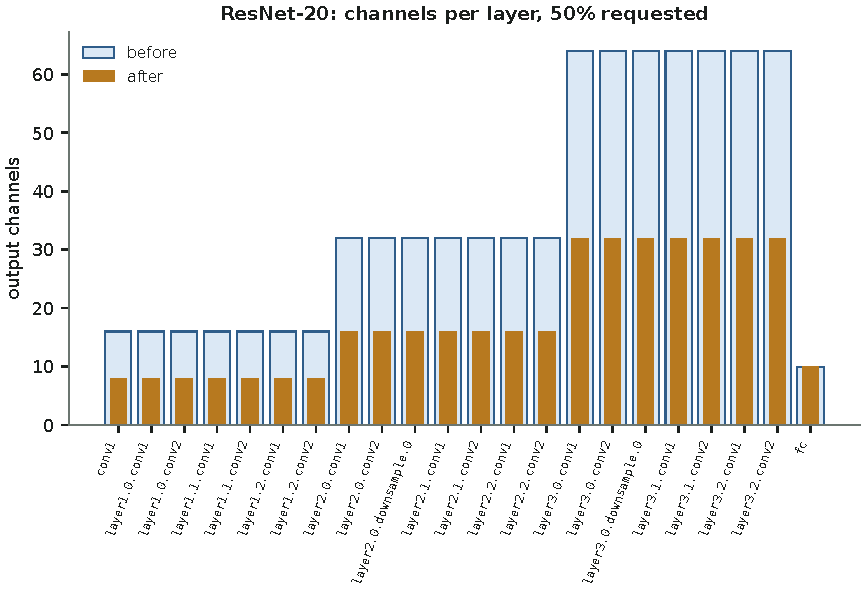
\includegraphics[width=0.62\textwidth]{fig_channels.pdf}
\caption{Output channels per layer of ResNet-20 before and after pruning.}
\label{fig:channels}
\end{figure}

\section{Gradual Pruning}
Fig.~\ref{fig:sawtooth} shows the accuracy after each cut and after each fine-tune for ResNet-20 and VGG-16-BN. Each cut drops accuracy and each fine-tune recovers most of it. On ResNet-20 the cuts reach 69.28\%, 63.36\% and 49.82\%, recovered to 87.63\%, 86.26\% and 83.97\%. On VGG-16-BN the cuts are gentler (91.34\% down to 86.66\%) and recover to 91.77\% down to 90.25\%; the over-parameterised network loses less per cut than the compact ResNet-20.

\begin{figure}[!htbp]
\centering
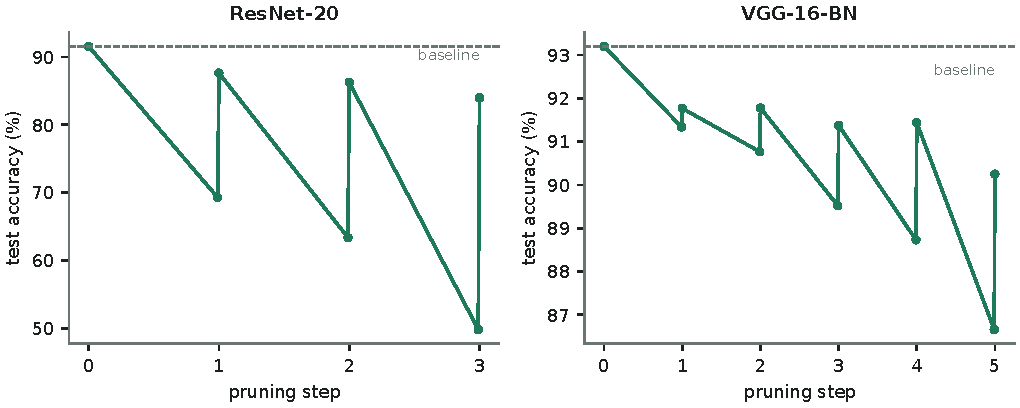
\includegraphics[width=0.75\textwidth]{fig_sawtooth.pdf}
\caption{Accuracy after each cut and after each fine-tune. ResNet-20 on Apple M5; VGG-16-BN transcribed from the Kaggle run.}
\label{fig:sawtooth}
\end{figure}

\subsection{Gradual against one-shot: a negative result}
At an equal total of six fine-tuning epochs, three steps of two epochs ended at 83.97\%, whereas one cut of the full 0.5 followed by six epochs ended at 85.03\% (Fig.~\ref{fig:oneshot}). One run each was made, so the 1.06-point difference is not established, but the data do not show gradual pruning to be better on this model and the report does not claim that it is. Gradual pruning is kept as an option because the budget search uses it in its recovery rung.

\begin{figure}[!htbp]
\centering
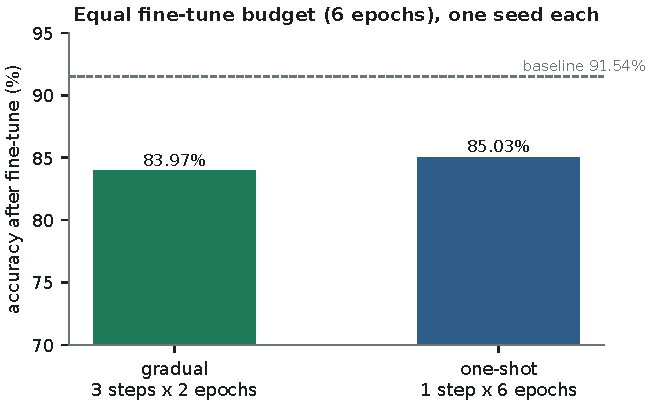
\includegraphics[width=0.42\textwidth]{fig_oneshot.pdf}
\caption{Gradual and one-shot pruning at the same fine-tune budget on ResNet-20, one seed each.}
\label{fig:oneshot}
\end{figure}

\section{Batch-Norm Re-estimation}
After a one-shot 0.5 cut with no fine-tuning, ResNet-20 falls from 91.54\% to 10.87\%, close to chance for ten classes. Re-estimating the batch-norm statistics from training batches raises it to 17.75\% (Fig.~\ref{fig:bn}). The left panel shows why the correction is needed: the running variance of the surviving channels of \code{layer1.0.bn1} after recalibration differs from the stale values copied from the old network. The correction is real but small; it does not replace fine-tuning, which is why distillation follows it in the pipeline.

\begin{figure}[!htbp]
\centering
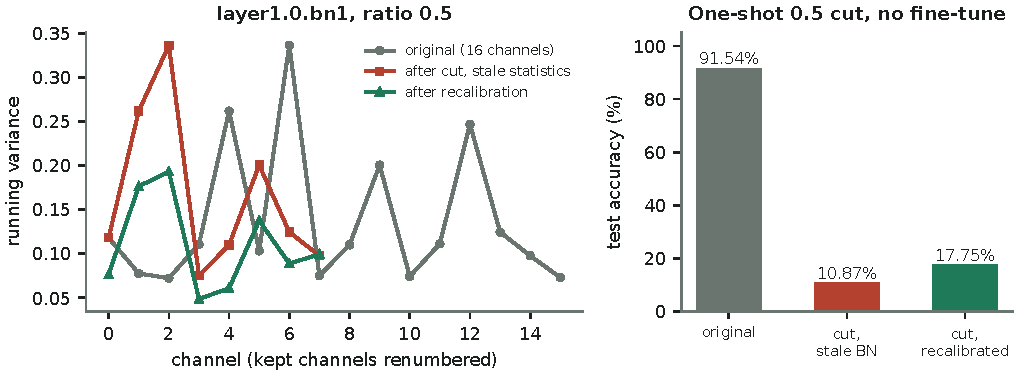
\includegraphics[width=0.8\textwidth]{fig_bn.pdf}
\caption{Running variance of one batch-norm layer before and after the cut (left) and the accuracy effect (right).}
\label{fig:bn}
\end{figure}

\section{Distillation Signal}
Fig.~\ref{fig:softmax} shows the teacher and student softmax outputs on one real test image of a cat, for the one-shot-pruned student that has not yet been fine-tuned. At temperature 1 the teacher gives 0.9991 to the true class and almost nothing elsewhere, so the other classes carry little information. At temperature 4 the teacher gives 0.7474 to cat and a visible ranking over the other nine classes; the student gives cat 0.0627 and favours horse. The NCKD term trains the student to reproduce the teacher's ranking over the non-target classes, and TCKD trains it on the target probability.

\begin{figure}[!htbp]
\centering
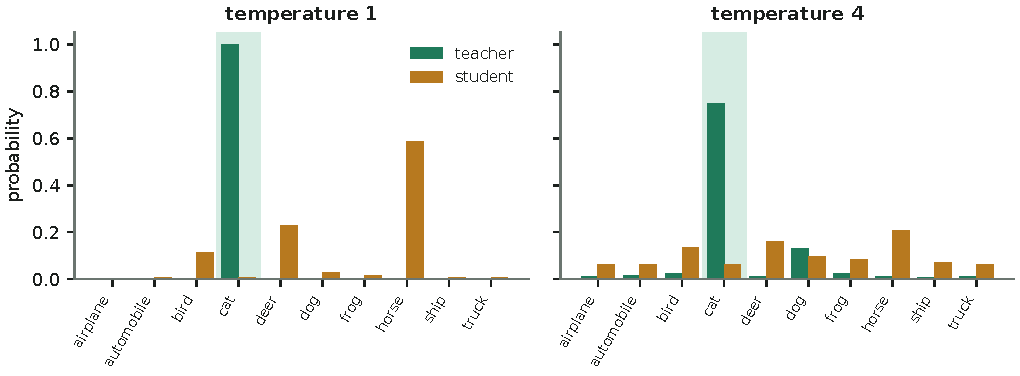
\includegraphics[width=0.8\textwidth]{fig_softmax.pdf}
\caption{Teacher and student softmax on one test image at temperature 1 (left) and 4 (right).}
\label{fig:softmax}
\end{figure}

\section{Quantization}
Fig.~\ref{fig:quant} shows one convolution of ResNet-20 (\code{layer2.0.conv1}, $32\times16\times3\times3$) before and after the INT8 round trip. The two histograms are nearly the same: the weight mean-squared error is $2.1\times10^{-7}$ and 248 of the 256 integer levels are used. The per-channel scales (right) differ across output channels by a factor of nearly two, which is why per-channel quantization is used rather than one scale for the whole tensor. In every run, all compute operators were quantized (22 of 22 for ResNet-20: 21 convolutions and one Gemm).

\begin{figure}[!htbp]
\centering
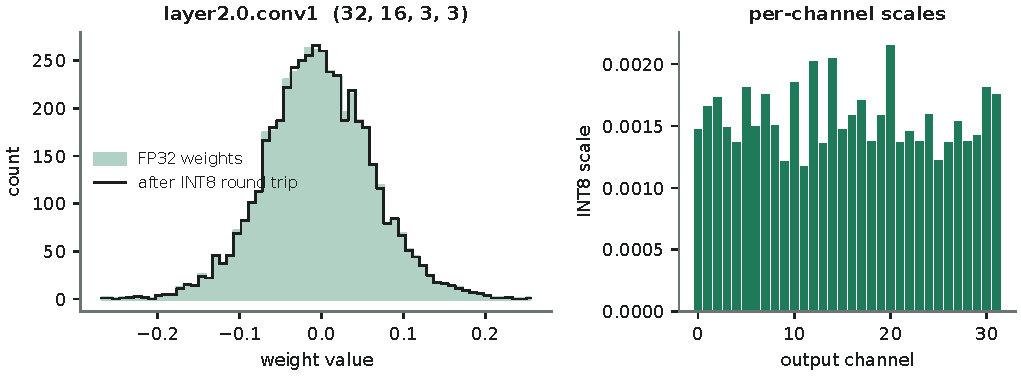
\includegraphics[width=0.8\textwidth]{fig_quant.pdf}
\caption{Weight histogram of one layer before and after INT8 (left) and the INT8 scale of each output channel (right).}
\label{fig:quant}
\end{figure}

\section{Layer Sensitivity}
Across the 22 layers of ResNet-20, quantization of a single layer produced an SQNR at the logits between 45.64 dB (\code{layer1.2.conv1}) and 62.34 dB (\code{layer3.2.conv2}), measured on four batches (Fig.~\ref{fig:sens}). The two most sensitive layers, \code{layer1.2.conv1} and \code{layer3.1.conv1}, are the ones the toolkit protects at a ratio of 0.5. The spread is 17 dB, so layers are not equally fragile and a single ratio for all layers leaves accuracy on the table.

\begin{figure}[!htbp]
\centering
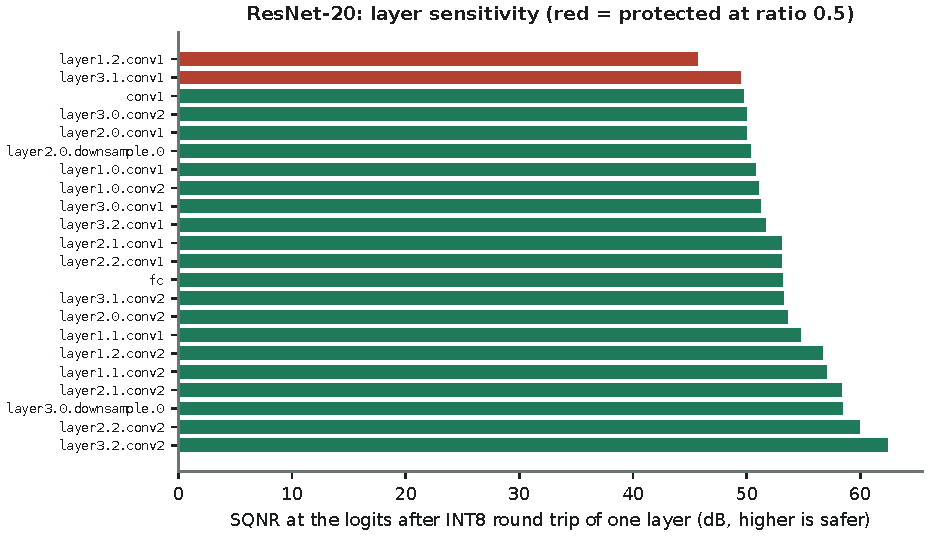
\includegraphics[width=0.6\textwidth]{fig_sens.pdf}
\caption{Per-layer SQNR of ResNet-20 after INT8 round trip of one layer at a time. Lower means more sensitive.}
\label{fig:sens}
\end{figure}

\section{Budget Search}\label{sec:search}
Three budgets were given to the search on ResNet-20 with shortened recovery schedules: 2 pruning steps of 1 fine-tune epoch, then 3 DKD distillation epochs, with 2 QAT epochs available as a fallback (Fig.~\ref{fig:search}, Table~\ref{tab:search}). In this first search, candidates were scored on the first $\sim$2,560 test images and the winner re-measured on all 10,000, so the search selected on the test set. Section~\ref{sec:valsearch} repeats it on a held-out validation split.

\begin{table}[!htbp]
\centering
\small
\begin{tabularx}{\textwidth}{@{}X X l r r@{}}
\toprule
Budget & Configuration chosen & Met & Accuracy (\%) & Latency (ms)\\
\midrule
accuracy drop $<1$ pp, size $<0.4$ MB & quantize only & yes & 91.54 & 0.878\\
latency $<0.45$ ms, drop $<8$ pp & prune 0.788, distill, quantize & yes & 84.96 & 0.361\\
latency $<0.02$ ms, drop $<0.5$ pp & best trade-off (same configuration) & no & 84.28 & 0.355\\
\bottomrule
\end{tabularx}
\caption{Outcomes of the budget search. The third budget is infeasible by design.}
\label{tab:search}
\end{table}

\begin{figure}[!htbp]
\centering
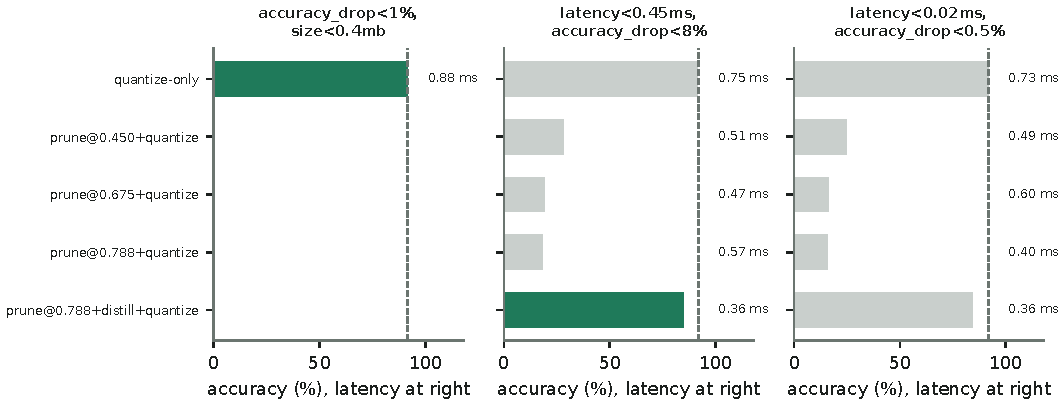
\includegraphics[width=0.8\textwidth]{fig_search.pdf}
\caption{Every attempt made under each budget. Green bars met the budget; the dashed line is the baseline accuracy.}
\label{fig:search}
\end{figure}

The second budget shows why the ladder exists. Quantization alone gave 0.747 ms, above the 0.45 ms limit. Pruning without recovery reached the latency range but collapsed accuracy to 18--28\%; only the rung that adds gradual fine-tuning with DKD met both limits. The third budget could not be met, and the search returned the most accurate candidate that came closest and said that the budget was missed. The ratio 0.788 is not a design choice: it is the third midpoint of a binary search over the requested channel ratio in $[0, 0.9]$ (0.45, 0.675, 0.788). It is a requested ratio. Alignment rounding and the protection of the two most sensitive layers at half the ratio mean the network that results is only about 8\% smaller in bytes than the headline 0.5 network (0.106 MB against 0.115 MB), so the effective ratio is far below 0.788. The 84.96\% of this run must not be compared with the headline 84.00\%: the schedules differ (this run adds three distillation epochs and per-layer protection), accuracy here was measured on a different subset with a different baseline (91.80\% against 91.54\%), and latency was timed in a different session. The measured latencies of the same file differ between searches (0.747 and 0.734 ms for quantize-only) because search-time measurements are short; borderline results are re-measured at full fidelity before being trusted.

\section{Budget Search on a Held-out Split}\label{sec:valsearch}
To remove the test-set selection of the previous section, ResNet-20 was retrained with the same recipe on 45,000 training images (91.67\% on the test set), 5,000 training images were held out, and the same three budgets were searched with candidates ranked and verdicts decided on those 5,000 images. The 10,000 test images scored only the configuration the search returned (Table~\ref{tab:valsearch}).

\begin{table}[!htbp]
\centering
\small
\setlength{\tabcolsep}{4pt}
\begin{tabularx}{\textwidth}{@{}X X l r r r@{}}
\toprule
Budget & Configuration returned & Met & Val.\ (\%) & Test (\%) & ms\\
\midrule
drop $<1$ pp, size $<0.4$ MB & quantize only & yes & 91.98 & 91.71 & 0.478\\
latency $<0.45$ ms, drop $<8$ pp & prune 0.225, distill, quantize & no & 90.26 & 89.77 & 0.519\\
latency $<0.02$ ms, drop $<0.5$ pp & prune 0.675, distill, quantize & no & 81.76 & 81.19 & 0.274\\
\bottomrule
\end{tabularx}
\caption{Budget search with selection on a held-out validation split (baseline 92.30\% validation, 91.67\% test). The third budget is infeasible by design.}
\label{tab:valsearch}
\end{table}

Two things change. The first budget is met by quantization alone as before, with the test accuracy (91.71\%) matching the baseline. The second budget, which the test-set search reported as met by pruning 0.788 with distillation, is \emph{not} met here: the best configuration reached 90.26\% on validation (89.77\% on test) but timed at 0.519 ms against a 0.45 ms limit, and quantization alone timed at 0.513 ms. The earlier verdict therefore depended on selecting on the test set and on a latency that moves from one session to the next: the same quantize-only file measured 0.747, 0.734, 0.478, 0.513 and 0.509 ms in different searches on the same laptop. A 0.45 ms limit sits inside that spread, so a pass or fail near it should not be read as a property of the method. What does hold in both searches is the ordering of the rungs: pruning without recovery collapses accuracy (27--47\% here), and only the distillation rung restores it.

\section{Verification of the Compressed ONNX File}
\code{experiments/verify\_onnx.py} runs the original PyTorch model and the compressed ONNX file on the same real CIFAR-10 test images. On all 10,000 test images the original ResNet-20 reached 91.54\% and the compressed file 84.00\%, a cost of 7.54 points that matches the pipeline's own measurement, and the two models gave the same prediction on 85.9\% of images. An earlier check on only the first 1,000 test images (in file order, not a random sample) gave 92.30\% and 83.20\%, a gap of 9.1 points; that slice is easier for the original model than the full set, so the full-set figure is the one to use. The file therefore works and is close to the original in the sense that matters for a deployed classifier, but it is not identical: the compressed model disagrees with the original on about one image in seven.

\section{Testing}
The toolkit has 172 automated tests in six files (core 104, pipeline 31, search 21, workflow 7, ImageNet-scale support 7, dataset registry 2), run by default, and one slow end-to-end test (train, gradual prune, INT8 quantize, report) that is deselected by default and takes about three and a half minutes. They cover the host probe, the alignment rule, dependency groups, the KD and DKD losses, budget parsing, the search ladder, ONNX export and the datasets. The stale-model defect of Section~\ref{sec:defect} is covered by a regression test.


\section{Limitations}
\begin{itemize}
\item The ResNet-56 rows of Table~\ref{tab:results} are a two-step, one-epoch smoke run, and its 11.27-point cost should not be read as the method's ability on this model. The full five-step schedule is reported separately in Table~\ref{tab:r56full}; it was run on a Kaggle CPU and transcribed from the notebook log.
\item The VGG-16-BN figures were transcribed from the Kaggle log and not loaded from the run's \code{results.json}; its latency is that of a Kaggle CPU without fast INT8.
\item Each experiment was run once; no confidence intervals are given, and differences of about one point (such as gradual against one-shot) are within what a different seed could change.
\item The ResNet-20 INT8 accuracy cost of 7.54 points is large. Longer fine-tuning or QAT may reduce it, but that was not measured here.
\item FP16 export, quantization-aware training, mixed-precision exclusion and latency-guided pruning are implemented and covered by correctness tests, but none was evaluated in the experiments above, so no claim is made about their benefit. The HAR path was not run to a result and is not part of the findings.
\item The 7.54-point ResNet-20 cost is a six-epoch result; the 25-epoch ResNet-56 run cost 3.90 points for the same parameter reduction.
\item Only residual and plain stacked CNNs on CIFAR-10 were tested. MobileNet-style depthwise networks and larger-resolution data were not.
\end{itemize}

% =====================================================================
\chapter{Conclusion and Future Scope}
\section{Summary}
CompressKit composes structured pruning, batch-norm re-estimation, distillation and quantization in a fixed order, measures everything on the exported ONNX file, and searches for the cheapest combination that meets a stated budget. Four mechanisms distinguish it from running the techniques separately: a host probe that gates INT8, a per-layer alignment rule, shared ratios across residual groups, and a label-free sensitivity ranking. On CIFAR-10, ResNet-20 became 9.1 times smaller and 3.2 times faster on an Apple M5 at a 7.54-point accuracy cost, and a VGG-16-BN run shrank 15.7 times at a 3.02-point cost.

\section{Conclusions}
\begin{itemize}
\item In these runs the accuracy cost came from pruning, not from INT8 quantization, which changed accuracy by at most 0.18 points.
\item Fine-tuning with distillation after each cut recovers most of the accuracy lost by that cut, but at an equal budget gradual pruning did not beat one-shot on ResNet-20.
\item Batch-norm re-estimation helps (10.87\% to 17.75\% after a 50\% cut) but is not a substitute for fine-tuning.
\item The budget search is useful because the cheap rungs often do not suffice: pruning without recovery reached lower latency and destroyed accuracy, and only the distillation rung restored it. On a held-out validation split the second budget (0.45 ms) was not met, and its latency limit lies inside the session-to-session timing spread of about 0.3 ms, so a single search near a limit is not conclusive.
\end{itemize}

\section{Future Scope}
\begin{itemize}
\item Run the full ResNet-56 schedule and the HAR ResNet-18 path on Kaggle, load the recorded \code{results.json} files, and repeat each experiment with several seeds to report variance.
\item Add support and tests for depthwise-separable networks such as MobileNet.
\item Evaluate QAT and longer fine-tuning on the 7.54-point ResNet-20 gap.
\item Add detection and segmentation models, and non-CPU runtimes with their own latency measurement.
\end{itemize}

% =====================================================================
{\footnotesize\setlength{\itemsep}{0pt}\setlength{\parskip}{0pt}
\begin{thebibliography}{99}
\bibitem{chae2026} W. Chae and K. Seo, ``Pipeline of Pruning, Knowledge Distillation, and Quantization for Model Compression,'' \emph{J. Electrical Engineering \& Technology}, vol. 21, pp. 2099--2105, 2026, doi: 10.1007/s42835-025-02541-7.
\bibitem{wang2025} Z. Wang, L. Shi, Z. Mei, X. Zhao, Z. Wang, and J. Li, ``Iterative knowledge distillation and pruning for model compression in unsupervised domain adaptation,'' \emph{Pattern Recognition}, vol. 164, art. 111512, 2025.
\bibitem{he2018} Y. He, J. Lin, Z. Liu, H. Wang, L.-J. Li, and S. Han, ``AMC: AutoML for Model Compression and Acceleration on Mobile Devices,'' in \emph{Proc. ECCV}, 2018.
\bibitem{zhou2026} M. Zhou, R. Mao, S. Sripada, and X. Li, ``AEMC: Aggregator-efficient model compression for streamlining LLMs,'' \emph{Neurocomputing}, vol. 672, art. 132779, 2026.
\bibitem{chen2021} W. Chen \emph{et al.}, ``Quantization of Deep Neural Networks for Accurate Edge Computing,'' \emph{ACM J. Emerging Technologies in Computing Systems}, vol. 17, no. 4, art. 54, 2021.
\bibitem{abdelsalam2025} R. Abdel-Salam, A. H. Abdel-Gawad, and A. G. Wassal, ``VLCQ: Post-training quantization for deep neural networks using variable length coding,'' \emph{Future Generation Computer Systems}, vol. 166, art. 107654, 2025.
\bibitem{khan2025} N. A. Khan and A. M. S. Rafat, ``Optimizing Deep Learning Models for Resource-Constrained Environments With Cluster-Quantized Knowledge Distillation,'' \emph{Engineering Reports}, vol. 7, art. e70187, 2025.
\bibitem{fang2026} X. Fang, L. Chen, H. Yin, X. Chen, and W. Wang, ``Communication Efficient Federated Learning With Quantization-Aware Training Design,'' \emph{IEEE Trans. Machine Learning in Communications and Networking}, vol. 4, pp. 45--59, 2026.
\bibitem{chen2020} Y. Chen, C. Li, L. Gong, X. Wen, Y. Zhang, and W. Shi, ``A deep neural network compression algorithm based on knowledge transfer for edge devices,'' \emph{Computer Communications}, vol. 163, pp. 186--194, 2020.
\bibitem{xu2024} L. Xu, J. Ren, Z. Huang, W. Zheng, and Y. Chen, ``Improving Knowledge Distillation via Head and Tail Categories,'' \emph{IEEE Trans. Circuits and Systems for Video Technology}, vol. 34, no. 5, pp. 3465--3478, 2024.
\bibitem{fang2023} G. Fang, X. Ma, M. Song, M. B. Mi, and X. Wang, ``DepGraph: Towards Any Structural Pruning,'' in \emph{Proc. IEEE/CVF CVPR}, 2023, pp. 16091--16101.
\bibitem{hinton2015} G. Hinton, O. Vinyals, and J. Dean, ``Distilling the Knowledge in a Neural Network,'' arXiv:1503.02531, 2015.
\bibitem{zhao2022} B. Zhao, Q. Cui, R. Song, Y. Qiu, and J. Liang, ``Decoupled Knowledge Distillation,'' in \emph{Proc. IEEE/CVF CVPR}, 2022, pp. 11953--11962.
\bibitem{he2016} K. He, X. Zhang, S. Ren, and J. Sun, ``Deep Residual Learning for Image Recognition,'' in \emph{Proc. IEEE CVPR}, 2016, pp. 770--778.
\bibitem{simonyan2015} K. Simonyan and A. Zisserman, ``Very Deep Convolutional Networks for Large-Scale Image Recognition,'' in \emph{Proc. ICLR}, 2015.
\bibitem{krizhevsky2009} A. Krizhevsky, ``Learning Multiple Layers of Features from Tiny Images,'' Tech. Rep., University of Toronto, 2009.
\bibitem{jacob2018} B. Jacob \emph{et al.}, ``Quantization and Training of Neural Networks for Efficient Integer-Arithmetic-Only Inference,'' in \emph{Proc. IEEE/CVF CVPR}, 2018, pp. 2704--2713.
\bibitem{bengio2013} Y. Bengio, N. L\'eonard, and A. Courville, ``Estimating or Propagating Gradients Through Stochastic Neurons for Conditional Computation,'' arXiv:1308.3432, 2013.
\end{thebibliography}}


\end{document}
